\hypersetup{pdfborder=0 0 0}

\section{Primary equations/conservation}
%\section{CROCO}

%%%%%%%%%%%%%%%%%%%%%%%%%%%%%%%%%%%%%%%%%%%%%%%%%%%%%%%%%%%%%%%%%%%%%%%%%%%%%
 %----------------------------------------------------------------------------
 \subsection{Continuous free-surface compressible equations in z-coordinates}
 %----------------------------------------------------------------------------
\label{subsectiongenesystem}

Conservation of mass, conservation of momentum (Newton's second law of motion), conservation of total energy (first law of thermodynamics) and conservation of chemical species are the backbones of ocean dynamics. In the ocean, the conservation of mass can be written as a prognostic equation for density (written $\rho$), the conservation of momentum leads to prognostic equations for the three components of momentum (written $\rho \mathbf{v}$) and the conservation of total energy can be stated as a prognostic equation for potential temperature ($\theta$). The conservation of chemical species can then be expressed as a prognostic equation for salinity ($S$). These conservation equations consequently lead to the following general system of prognostic equations (expressed in flux form):
\begin{subequations}
 \begin{alignat}{2}
 \displaystyle
 \label{NS_a} 
 & \frac{\partial\rho}{\partial t} &&= - \mathbf{\nabla}\cdot(\rho \mathbf{v})\\[3mm]  
 \label{NS_b}
 & \frac{\partial \rho \mathbf{v}}{\partial t} 
	 &&= -\mathbf{\nabla}\cdot(\rho \mathbf{v}\otimes \mathbf{v}) 
	  \color{black} -2\rho\ \mathbf{\Omega}\ \times \ \mathbf{v} \color{black} -\mathbf{\nabla}p + 		
	\mathbf{\nabla}\cdot\left(
	\mu(\mathbf{\nabla}\mathbf{v}+\mathbf{\nabla}\mathbf{v}^{\ T})
 +\mu_2(\mathbf{\nabla}\cdot\mathbf{v})\ \mathbf{I}\ \right)
 +\rho \mathbf{g}\\
 %
 \label{NS_c}
 & \frac{\partial \rho \theta}{\partial t} &&=-\mathbf{\nabla}\cdot(\rho \theta\mathbf{v})
 +\mathbf{\nabla}\cdot\color{black}(\kappa_\theta\mathbf{\nabla}{\theta})\color{black}\\[3mm]
 %
 \label{NS_d}
 & \frac{\partial \rho S}{\partial t} &&=-\mathbf{\nabla}\cdot(\rho S\mathbf{v})
 +\mathbf{\nabla}\cdot\color{black}(\kappa_S\mathbf{\nabla}{S})\color{black}
 %
  \end{alignat}
\end{subequations}
with $\mu$, $\mu_2$, $\kappa_T$ and $\kappa_S$ respectively the dynamical and bulk viscosities and the thermal and salt diffusivities. $\mathbf{\Omega}$ is the earth instant rotation vector.
Assuming that variables are in thermodynamic equilibrium, the equation of state (EOS) can be formulated as a non-linear, diagnostic functional relation between temperature, salinity, density and (total) pressure (written $p$):
\begin{equation}
 \label{NS_e}
 \rho = \rho_{eos}[\theta,S,p]
\end{equation}

\color{red}
In Cartesian coordinates, a simple, incompressible evolution of $\rho$ is given by:
\begin{equation}
\displaystyle
\frac{d \rho}{d t}=
\frac{\partial}{\partial x} \bigg(\kappa_\rho^h \frac{\partial \rho}{\partial x}\bigg\rvert_{tz}\bigg)_{tz}
+ \frac{\partial}{\partial z} \bigg( \kappa_\rho^v \frac{\partial \rho}{\partial z}\bigg\rvert_{tx}\bigg)_{tx} 
\label{eq_diff_cart}
\end{equation}
where $\kappa_\rho^h$ and $\kappa_\rho^v$ are the (horizontal and vertical) diffusivities of density.
\color{black}

The position of the interface separating the ocean and the atmosphere must additionally be calculated and is introduced as a boundary condition. This can be achieved by stating that a salty-water particles that is just bellow this interface in the ocean, remains at the interface, leading to the surface kinematic relation:
\begin{equation}
  \displaystyle
  \label{NS_BC2}
  %\frac{\textrm{d}\zeta(\mathbf{x}_{\scriptscriptstyle H},t)}{\textrm{dt}}=w(\mathbf{x}_{\scriptscriptstyle H},z=\zeta)
  \frac{\partial \zeta}{\partial t}=w(\mathbf{x}_{\scriptscriptstyle H},z=\zeta)-\mathbf{v}_H(\mathbf{x}_{\scriptscriptstyle H},z=\zeta)\cdot\mathbf{\nabla}_H\zeta
\end{equation}
where $\zeta$ is the free-surface anomaly in the vicinity of the geoid and subscribe $H$ indicates that only the horizontal component is considered. Assuming then that ocean water cannot penetrate the ocean bottom (at depth $z=-H$):
\begin{equation}
 \displaystyle
 \label{NS_BC0}
  \mathbf{v}(\mathbf{x}_{\scriptscriptstyle H},z=-H)=\mathbf{0}
\end{equation}
Neglecting surface-tension pressure drop, the boundary condition for pressure at the surface of the ocean is given by:
\begin{equation}
 \displaystyle
 \label{NS_BC1}
  p(\mathbf{x}_{\scriptscriptstyle H},z=\zeta,t)= p_{atm}
\end{equation}
with $p_{atm}$ the atmospheric pressure above the surface of the ocean.
The resulting system of prognostic equations, diagnostic relations and boundary conditions leads to a non-linear problem whose main characteristics is the wild spectrum of dynamic processes involved (see for instance \cite{gill_atmosphere-ocean_1982} or \cite{vallis_atmospheric_2006}). Periodic processes such as ocean waves can give a comprehensive overview of the extension of space-time spectrum of transient processes which can propagate in the ocean and \cite{auclair_modied_2021} derive a compressible, free-surface, stratified model of two dispersion relations for wave-numbers and pulsation gathering acoustic, surface and internal waves and insisting on the modification of the dispersion of gravity (acoustic) waves by compressibility (gravity and stratification).\\
Formulated thus, the system of Navier-Stokes and conservation equations for a free-surface ocean can, at least in theory, be integrated straightforwardly. All variables but the pressure have their own prognostic equation and pressure can be diagnosed from the EOS \ref{NS_e}. Note that the system can be reformulated so that pressure is also given by a prognostic equation.
 %----------------------------------------------------------------------------  
 %\subsection{Density and pressure decomposition}
 %----------------------------------------------------------------------------
 
 \subsection{Terrain-following coordinates}

 %%%%%%%%%%%%%%%%%%%%%%%%%%%%%%%%%%%%%%%%%%%%%%%%%%%%%%%%%%%%%%%%%%%%%%%%%%%%%
\subsubsection{Definition}
%%%%%%%%%%%%%%%%%%%%%%%%%%%%%%%%%%%%%%%%%%%%%%%%%%%%%%%%%%%%%%%%%%%%%%%%%%%%%
The capacity of numerical models to portray the evolution of global or regional oceanic circulation relies on horizontal and vertical definition of a grid on which the Navier-Stokes and conservation equations previously defined are solved and integrated in time.

Due to considerations of the representation of bathymetric features, terrain-following coordinates, or S-coordinates, can be chosen for the vertical discretisation. They are generally defined based on "generalized surfaces" $s=cte$ with s given by:
\begin{equation}
 \displaystyle
 s=s(x,y,z,t)
\end{equation}
requiring:
\begin{equation}
 \displaystyle
 \frac{\partial s}{\partial z}\bigg\vert_{xyt}\ne 0
\end{equation}
As a consequence, for $\partial s / \partial z$ to be continuous and single-signed/either strictly positive or negative, $s(z)$ must be monotonic.

%%%%%%%%%%%%%%%%%%%%%%%%%%%%%%%%%%%%%%%%%%%%%%%%%%%%%%%%%%%%%%%%%%%%%%%%%%%%%
%\subsubsection{Examples}
%%%%%%%%%%%%%%%%%%%%%%%%%%%%%%%%%%%%%%%%%%%%%%%%%%%%%%%%%%%%%%%%%%%%%%%%%%%%%
Several examples and comparisons on the choice of $s(x,y,z,t)$ are given in chapter 6 of \citet{griffies_fundamentals_2004}.

Following  \citep{shchepetkin_regional_2005},  $\sigma$-coordinates can for instance be defined by:
\begin{equation}
 \displaystyle
 z(\mathbf{x},\sigma,t)=\sigma H(\mathbf{x})
\end{equation}
or:
\begin{equation}
 \displaystyle
 z(\mathbf{x},\sigma,t)=\sigma(H+\zeta)+\zeta
\end{equation}
Where $H(\mathbf{x})$ is the bottom topography and $\zeta(\mathcal{x},t)$ the surface elevation anomaly. Its generalization to s-coordinates is defined by:
\begin{equation}
 \displaystyle
 z(\mathbf{x},s,t)=\mathcal{S}(s) H(\mathbf{x})
\end{equation}
which is currently written:
\begin{equation}
 \displaystyle
 z(\mathbf{x},\sigma,t)=\mathcal{S}(\sigma) H(\mathbf{x})
\end{equation}
where $s(\sigma)$ can be a non-linear function. Some current definitions are presented on the Wiki-Roms web-site \footnote{\url{https://www.myroms.org/wiki/Vertical_S-coordinate}}.\\


%%%%%%%%%%%%%%%%%%%%%%%%%%%%%%%%%%%%%%%%%%%%%%%%%%%%%%%%%%%%%%%%%%%%%%%%%%%%%
\subsubsection{Vertical velocities}
%%%%%%%%%%%%%%%%%%%%%%%%%%%%%%%%%%%%%%%%%%%%%%%%%%%%%%%%%%%%%%%%%%%%%%%%%%%%%

Using coordinate transformation presented in \ref{annexe_coordS}, the vertical velocity $w \equiv v_z$ is decomposed as :
\begin{subequations}
  \begin{alignat}{2}
  \displaystyle 
	& v_z &&\equiv \frac{d z}{d t}\\
	& &&=\underbrace{\underbrace{\frac{\partial z}{\partial s}\bigg\rvert_{tx}}_{\equiv h} \frac{d s}{dt}}_{\equiv v_s}
	+\underbrace{\frac{\partial z}{\partial x}\bigg\rvert_{ts} \underbrace{\frac{d x}{dt}}_{\equiv u}
	+\frac{\partial z}{\partial t}\bigg\rvert_{xs} \underbrace{\frac{d t}{dt}}_{=1}}_{=\frac{dz}{dt}\big\rvert_{s}}\\
	& &&=\frac{\partial z}{\partial s}\bigg\rvert_{tx} \frac{d s}{dt}
	+\frac{d z}{d t}\bigg\rvert_{s} \\
	& &&=\ \ h \frac{d s}{dt}\quad
	+\frac{d z}{d t}\bigg\rvert_{s}\\
	& &&=
	\ \ v_s 
	\qquad+\underbrace{\frac{\partial z}{\partial t}\bigg\rvert_{xs}
	+u \frac{\partial z}{\partial x}\bigg\rvert_{ts}}
	_{\frac{d z}{d t}\big\rvert_{s}=v_{\Sigma,z}}
  \end{alignat}
  \label{eq_vertvelcomp}
\end{subequations}
where:
\begin{equation}
	\displaystyle
	h\equiv\frac{\partial z}{\partial s}\bigg\rvert_{tx} 
	v_s\equiv h\frac{d s}{d t}
\end{equation}

In other words, the vertical velocity is the composition of $v_{\Sigma,z}$ the vertical component of the velocity of the moving surface $s=cst$, and $v_s$ the velocity through this same surface.

%%%%%%%%%%%%%%%%%%%%%%%%%%%%%%%%%%%%%%%%%%%%%%%%%%%%%%%%%%%%%%%%%%%%%%%%%%%%%%
%\subsubsection{Vertical velocities in $"\sigma"$-coordinates}
%%%%%%%%%%%%%%%%%%%%%%%%%%%%%%%%%%%%%%%%%%%%%%%%%%%%%%%%%%%%%%%%%%%%%%%%%%%%%
In the more restrictive case when $\sigma$-coordinates are used:
% In $\sigma$-coordinates:
\begin{equation}
 \displaystyle
 \sigma=\frac{z-\zeta}{H+\zeta}
\end{equation}
and as a consequence:
\begin{equation}
 \displaystyle
 v_z=w=\mathbf{u}_z.\mathbf{v}
=\frac{dz}{dt}=\underbrace{(H+\zeta)\frac{d\sigma}{dt}}_{\equiv v_{\sigma}}
 +(\sigma-1)\frac{dH}{dt}
 +\sigma\frac{d\zeta}{dt}
\end{equation}
where in $\sigma$-coordinates:
\begin{equation}
 \displaystyle
v_{\sigma}=(H+\zeta)\frac{d\sigma}{dt}
\end{equation}

%%%%%%%%%%%%%%%%%%%%%%%%%%%%%%%%%%%%%%%%%%%%%%%%%%%%%%%%%%%%%%%%%%%%%%%%%%%%%
\subsubsection{Divergence of the velocity field in s-coordinates}
%%%%%%%%%%%%%%%%%%%%%%%%%%%%%%%%%%%%%%%%%%%%%%%%%%%%%%%%%%%%%%%%%%%%%%%%%%%%%
Using :
\begin{equation}
 \displaystyle
 \frac{\partial}{\partial t} \frac{\partial z}{\partial s}\bigg\vert_{tx}= \frac{\partial h}{\partial t} \qquad and \qquad \frac{\partial}{\partial x} \frac{\partial z}{\partial s}\bigg\vert_{tx}= \frac{\partial h}{\partial x}
\end{equation}
%and
%\begin{equation}
% \displaystyle
% \frac{\partial}{\partial x} \frac{\partial z}{\partial s}\bigg\vert_{tx}= \frac{\partial h}{\partial x}
%\end{equation}
%
the expression of the divergence in s-coordinates is given by:
\begin{subequations}
  \begin{alignat}{2}
  & h \ \mathbf{\nabla}.( \mathbf v) &&= h \frac{\partial u}{\partial x} \bigg \rvert_{zt} +h \frac{\partial v_z}{\partial z} \bigg \rvert_{xt}\\ 
  & && = h \frac{\partial u}{\partial x} \bigg \rvert_{st} - \frac{h}{h} \frac{\partial u}{\partial s}\bigg \rvert_{tx} \frac{\partial z}{\partial x}\bigg \rvert_{ts} \\
  & && \quad + \frac{h}{h}  \frac{\partial}{\partial s} \bigg ( v_s + \frac{\partial z }{\partial t}\bigg \rvert_{xs} + u \frac{\partial z}{\partial x}\bigg \rvert_{ts} \bigg )\\
  & && = h \frac{\partial u}{\partial x} \bigg \rvert_{st} -  \frac{\partial u}{\partial s}\bigg \rvert_{tx} \frac{\partial z}{\partial x}\bigg \rvert_{ts} \\
  & && \quad +  \frac{\partial v_s}{\partial s} +  \frac{\partial h}{\partial t} + u \frac{\partial h}{\partial x} + \frac{\partial u}{\partial s}\bigg \rvert_{tx} \frac{\partial z}{\partial x}\bigg \rvert_{ts}\\
  & && = \frac{\partial v_s}{\partial s}\bigg \rvert_{tx} + \frac{\partial h u}{\partial x} \bigg \rvert_{ts}+ \frac{\partial h}{\partial t}\bigg \rvert_{xs}
  \end{alignat}
\end{subequations}
Note that this is a particular case of the formulation of a change of variables with its Jacobian ($J=h$ in the present case). %This leads to several useful conservative formulations in the following section.
%


%%%%%%%%%%%%%%%%%%%%%%%%%%%%%%%%%%%%%%%%%%%%%%%%%%%%%%%%%%%%%%%%%%%%%%%%%%%%%
\subsubsection{(local) Conservative "flux" forms: kinematics \& dynamics}
%%%%%%%%%%%%%%%%%%%%%%%%%%%%%%%%%%%%%%%%%%%%%%%%%%%%%%%%%%%%%%%%%%%%%%%%%%%%%
Two general conservative formulations can be obtained combining this with the continuity equation \citep{auclair_woceanfr_2011}\footnote{WOcean.fr Web Site: \url{http://poc.omp.obs-mip.fr/auclair/WOcean.fr/SNH/Restricted/NH-NBQ/Sources/Images/png/Coord_demo.png}}.

$A$ is a property given per unit mass (thermodynamically intensive) (see the demonstration on web site). The first two (conservative) relations are fundamentals to  analytical and numerical modeling.\\

\textbf{\textit{Based on the conservation of mass:}}
\begin{equation}
  \displaystyle 
  \rho \frac{d A}{dt}
  =\frac{\partial \rho A}{\partial t}\bigg\rvert_{xz}
  +\frac{\partial \rho A u}{\partial x}\bigg\rvert_{tz}
  +\frac{\partial \rho  v_s}{\partial z}\bigg\rvert_{tx}
\end{equation}

\textbf{\textit{Based on the conservation of mass \& in s-coordinates:}}
\begin{equation}
  \displaystyle 
  \rho h \frac{d A}{dt}
  =\frac{\partial \rho h A}{\partial t}\bigg\rvert_{xs}
  +\frac{\partial \rho h A u}{\partial x}\bigg\rvert_{ts}
  +\frac{\partial \rho  A v_s}{\partial s}\bigg\rvert_{tx}
\end{equation}
\textbf{\textit{A kinematic, non-conservative formulation}} can be obtained without the continuity equation:
\begin{equation}
\frac{d A}{d t} = \frac{\partial A}{\partial t} \bigg\rvert_{xs} + u \frac{\partial A}{\partial x} \bigg\rvert_{ts} + \frac{v_s}{h}\frac{\partial A}{\partial s}\bigg\rvert_{tx}
\end{equation}
The demonstration is given in \citep{auclair_woceanfr_2011}\footnote{WOcean.fr Web Site: \url{http://poc.omp.obs-mip.fr/auclair/WOcean.fr/SNH/Restricted/NH-NBQ/Sources/Images/png/Coord_demo.png}}.\\

\textbf{\textit{Conservation of mass:}}
note finally that the conservation of mass $A=1$ can then be rewritten:
\begin{equation}
  \displaystyle 
  \label{mass_s}
  h\frac{d\rho}{d t}
  =\frac{\partial \rho h }{\partial t}\bigg\rvert_{xs}
  +\frac{\partial \rho h u}{\partial x}\bigg\rvert_{ts}
  +\frac{\partial \rho  v_s}{\partial s}\bigg\rvert_{tx}
\end{equation}

Additionnally, the evolution of $\rho$ in equation \ref{eq_diff_cart} can be rewritten in s-coordinates as:
\begin{equation}
\label{eq_diff_s}
\displaystyle
h \frac{d \rho }{d t} \approx
\frac{\partial}{\partial x} \bigg(h \kappa^h \frac{\partial \rho}{\partial x}\bigg\rvert_{ts}\bigg)_{ts}
+ \frac{\partial}{\partial s} \bigg(\frac{\kappa^v}{h} \frac{\partial \rho}{\partial s}\bigg\rvert_{tx}\bigg)_{tx} 
\end{equation}
with: $\kappa_c^h \approx \kappa^h$ and $\kappa_c^v \approx \kappa^v$.\\

%%%%%%%%%%%%%%%%%%%%%%%%%%%%
\subsubsection{Conservation of an extensive quantity in a free-surface ocean}
%%%%%%%%%%%%%%%%%%%%%%%%%%%

We want to specify the conservation of an extensive property defined as $\mathcal{A}=\iiint_{\mathcal{V}(t)} \rho A d\tau$, in a region of the ocean with a varying free-surface.

For a time-dependant volume $\mathcal{V}(t)$ moving with a velocity $\mathbf{v}_{\Sigma}$, a formulation of the Reynolds transport theorem (or Leibnitz theorem) is \citep{truesdell_classical_1960}:

\begin{subequations}
  \begin{alignat}{2}
  \displaystyle 
  &  \frac{d}{dt} \iiint_{\mathcal{V}(t)} \rho A d\tau && =
  \iiint_{\mathcal{V}(t)} \frac{D\rho A}{Dt}  d\boldsymbol{x}
  +\iiint_{\mathcal{V}(t)} \rho A \mathbf{\nabla}.\mathbf{v}_{\Sigma}\ d\mathbf{x}\\
 & && =
  \iiint_{\mathcal{V}(t)} \frac{\partial \rho A}{\partial t}\bigg\rvert_{xz} d\tau
  %+ \varoiint_{\mathcal{V}(t)}\rho A \mathbf{v}.\mathbf{S}\\
  + \oiint_{\mathcal{S}(t)}\rho A   \mathbf{v}_{\Sigma}.\mathbf{n}_{\Sigma}dS_{\Sigma}
  \end{alignat}
\end{subequations}
With the material derivate $D/Dt$ here associated to $  \mathbf{v}_{\Sigma}$:
\begin{equation}
 \displaystyle
 \frac{D\bullet}{Dt}=\frac{\partial \bullet}{\partial t}\bigg\vert_{\boldsymbol{\xi}}
 +  \mathbf{v}_{\Sigma}.\mathbf{\nabla}_{t,\boldsymbol{\xi}}\bullet
\end{equation}

In oceanic case, $\mathcal{V}(t)$ is taken as $\mathcal{V}_s$ a sum of water columns. Absant shoaling processes (banc découvrant???), this volume's boundaries only move in the vertical direction with the elevation of the free-surface. It is then possible to express $\mathcal{A}$ in s-coordinates with the Jacobian $\mathcal{J}=h$:

\begin{equation}
  \displaystyle 
 	\frac{d }{d t} \iiint_{\mathcal{V}_{s}} \rho A\ d\tau  =
 	\frac{d }{d t} \iiint_{\mathcal{V}_{s}} \rho A\ h ds dx_s dy_s
\end{equation}

In this case, with the definition of surface $s=cst$, the boundaries of volume $\mathcal{V}_s$ are constant and the time-derivative can directly be applied through the integral as :
\begin{subequations}
  \begin{alignat}{2}
  \displaystyle 
   &\frac{d }{d t} \iiint_{\mathcal{V}_{s}} \rho A\ h ds dx_s dy_s && =
   \iiint_{\mathcal{V}_{s}} \frac{\partial h \rho A}{\partial t}\bigg \vert_s ds dx_s dy_s\\
   & &&= \iiint_{\mathcal{V}_{s}} \rho h \frac{\partial A}{\partial t}\bigg \vert_s  ds dx_s dy_s + \iiint_{\mathcal{V}_{s}} A \frac{\partial \rho h}{\partial t}\bigg \vert_s ds dx_s dy_s \\
   \end{alignat}
\end{subequations}

This formulation is found following Reynolds transport theorem in annex \ref{annexe_reynolds}.

In which can use the conservation of mass in equation \ref{mass_s} and the formulation of evolution of $\rho$ in equation \ref{eq_diff_s} :
\begin{subequations}
  \begin{alignat}{2}
  \displaystyle 
   & \frac{d }{d t} \iiint_{\mathcal{V}_{s}} \rho A\ h ds dx_s dy_s && = \iiint_{\mathcal{V}_{s}} \frac{\partial A}{\partial t}\bigg \vert_s \rho h ds dx_s dy_s\\
 & && \quad - \int_x \int_{-1}^0 A \frac{\partial \rho h u}{\partial x}\bigg\rvert_{ts} \ dx ds \\ 
 & && \quad - \int_x \int_{-1}^0 A \frac{\partial \rho v_s}{\partial s}\bigg\rvert_{tx} \ dx ds \\
 & && \quad + \int_x \int_{-1}^0 A \frac{\partial}{\partial x} \bigg(h \kappa^h \frac{\partial \rho}{\partial x}\bigg\rvert_{ts}\bigg)_{ts} \ dx ds \\
 & && \quad + \int_x \int_{-1}^0 A \frac{\partial}{\partial s} \bigg(\frac{\kappa^v}{h} \frac{\partial \rho}{\partial s}\bigg\rvert_{tx}\bigg)_{tx} \ dx ds 
   \end{alignat}
\end{subequations}

Simplifying the fluxes \color{red}(revoir alignement, manque des dy( est passé en 2D), Notation bornes dimension vertical (soit de -1 à 0, soit de 0 à 1...))\color{black}:
\begin{subequations}
  \begin{alignat}{2}
& \frac{d }{d t} \iiint_{\mathcal{V}_{s}} \rho A\ h ds dx_s dy_s &&=  \int_x \int_{-1}^0 \rho h \frac{\partial A}{\partial t}\bigg\rvert_{xs} \ dx ds\\
 & && \quad - \int_x \int_{-1}^0 \frac{\partial \rho h A u}{\partial x}\bigg\rvert_{ts} \ dx ds
 + \int_x \int_{-1}^0\rho h u \frac{\partial A}{\partial x}\bigg\rvert_{ts} \ dx ds\\ 
 & && \quad - \int_x \int_{-1}^0 \frac{\partial \rho A v_s}{\partial s}\bigg\rvert_{tx} \ dx ds
 + \int_x \int_{-1}^0 \rho v_s \frac{\partial A}{\partial s}\bigg\rvert_{tx} \ dx ds \\
 & && \quad + \int_x \int_{-1}^0 \frac{\partial}{\partial x} \bigg(h A \kappa^h \frac{\partial \rho}{\partial x}\bigg\rvert_{ts}\bigg)_{ts} \ dx ds 
 - \int_x \int_{-1}^0 h \kappa^h \frac{\partial A}{\partial x}\bigg\rvert_{ts} \frac{\partial \rho}{\partial x}\bigg\rvert_{ts} \ dx ds \\
 & && \quad + \int_x \int_{-1}^0 \frac{\partial}{\partial s} \bigg( A \frac{\kappa^v}{h} \frac{\partial \rho}{\partial s}\bigg\rvert_{tx}\bigg)_{tx} \ dx ds 
 - \int_x \int_{-1}^0 \frac{\kappa^v}{h} \frac{\partial A}{\partial s}\bigg\rvert_{tx} \frac{\partial \rho}{\partial s}\bigg\rvert_{tx} \ dx ds 
  \end{alignat}
\end{subequations}
This leads to :
\begin{subequations}
  \begin{alignat}{2}
  \displaystyle 
  &\frac{d }{d t} \int_x \int_{-1}^0 \rho h A\ dx ds &&=
 %
 % Begin 5th line
 %
\quad  \int_x \int_{-1}^0 \rho h \frac{\partial A}{\partial t}\bigg\rvert_{ts} \ dx ds\\
 & && \quad - \bigg[ \int_{-1}^0 \rho h A u \ ds\bigg]_{x}
 + \int_x \int_{-1}^0\rho h u \frac{\partial A}{\partial x}\bigg\rvert_{ts} \ dx ds\\ 
 & && \quad - \bigg[ \int_{x} \rho A v_s \ ds\bigg]_{0}^1
 + \int_x \int_{-1}^0 \rho v_s \frac{\partial A}{\partial s}\bigg\rvert_{ts} \ dx ds \\
 & && \quad + \bigg[ \int_{-1}^0 h A \kappa^h \frac{\partial \rho}{\partial x}\bigg\rvert_{ts} \ ds \bigg]_{x}
 - \int_x \int_{-1}^0 h \kappa^h \frac{\partial A}{\partial x}\bigg\rvert_{ts} \frac{\partial \rho}{\partial x}\bigg\rvert_{ts} \ dx ds \\
 & && \quad + \bigg[ \int_x A \frac{\kappa^v}{h} \frac{\partial \rho}{\partial s}\bigg\rvert_{tx} \ dx \bigg]_0^1
 - \int_x \int_{-1}^0 \frac{\kappa^v}{h} \frac{\partial A}{\partial s}\bigg\rvert_{tx} \frac{\partial \rho}{\partial s}\bigg\rvert_{tx} \ dx ds \\
 %
 % Begin 6th line
 %
 & &&= \quad  \int_x \int_{-1}^0 \rho h \frac{d A}{d t} \ dx ds\\
 & && \quad - \bigg[ \int_{-1}^0 \rho h A u \ ds\bigg]_{x} - 0\\ 
 & && \quad + \bigg[ \int_{-1}^0 h A \kappa^h \frac{\partial \rho}{\partial x}\bigg\rvert_{ts} \ ds \bigg]_{x}
 - \int_x \int_{-1}^0 h \kappa^h \frac{\partial A}{\partial x}\bigg\rvert_{ts} \frac{\partial \rho}{\partial x}\bigg\rvert_{ts} \ dx ds \\
 & && \quad + \bigg[ \int_x A \frac{\kappa^v}{h} \frac{\partial \rho}{\partial s}\bigg\rvert_{tx} \ dx \bigg]_0^1
 - \int_x \int_{-1}^0 \frac{\kappa^v}{h} \frac{\partial A}{\partial s}\bigg\rvert_{tx} \frac{\partial \rho}{\partial s}\bigg\rvert_{tx} \ dx ds 
  \end{alignat}
\end{subequations}


With $\bigg[ \int_{x} \rho A v_s \ ds\bigg]_{0}^1 = 0$ since $v_s$ is void at the bottom and top boundary. 

%\subsection{S-coordinates}
%Integration over the water column whose surface is varying in time. 
%A key property is:
%\begin{equation}
% \displaystyle
% \frac{dh}{dt}(t,\mathbf{x},z)=\frac{d}{dt}\left( \frac{\partial z}{\partial s}\bigg\vert_{txy}\right)
% =\frac{\partial }{\partial s}\frac{dz}{dt}=\frac{\partial w}{\partial s}(t,\mathbf{x},z)
%\end{equation}

























 \subsection{Conservation of potential energy and decomposition in free-surface ocean}
 
 \subsubsection{Definition of APE and BPE}
 
 %%%A remplir blabla Winters etc.
 
 
 \subsubsection{Reference state(s)}
 
\cite{saenz_estimating_2015} and more generally Tailleux in his latest publications \citep{tailleux_local_2018} insist on the fact that Lorenz reference state is difficult to define and compute... As a consequence, these studies are dedicated to the evaluation of the errors and discrepancies when simpler and easier-to-obtain reference states are defined (horizontal averaged...). \cite{saenz_estimating_2015} additionally describes in detail an algorithm to compute Lorenz' reference state in an efficient way. They associate the computation of $Z_r(\rho)$ from the computation of the Level of Neutral Buoyancy (their LNB) and they separate it from the computation of Lorenz' reference state that is computed first by inverting a non-linear relation... This algorithm is claimed to be much more efficient that classical redistribution adiabatic algorithms based on \citep{winters_available_1995}.\\
Behind the reference state and more precisely behind the reference profile, several ideas:
\begin{itemize}
	\item A basic (not necessarily resting but possibly balanced) state to which full dynamics is to be compared,
	\item The Boussinesq assumption based on the choice of a reference (constant) density (named here $\tilde{\rho}_{0}$ that is subtracted from the 3D total density. An hydrostatic pressure $p_{00}$ is defined by $\partial p_{00}/ \partial z=-\tilde{\rho}_{0} g$. Subtracting directly a vertically-varying reference density $\tilde{\rho}_{0}(z)$ leads to the less restrictive anelastic assumption. Interestingly enough, this Boussinesq reference state $(\tilde{\rho}_{0},\ p_{00})$ can be associated to the thermodynamic equilibrium state. \cite{tailleux_energetics_2009,tailleux_thermodynamicsdynamics_2012} associate this reference state to the \textit{internal dead energy} compartment (named $IE0$) concluding that "the viscous dissipation of KE and the diffusive dissipation of APE" increases the reference temperature $T_{00}$ (decreasing $\tilde{\rho}_{0}$) by increasing the IE0 (page 9 of the latter publication).
	\item The reference profile (named here $\rho_0$) with both time and space (vertical) dependencies is then defined by $\rho(t,\mathbf{x})=\tilde{\rho}_{0}+\rho_0(t,z)+\rho'(t,\mathbf{x})$.  \cite{tailleux_thermodynamicsdynamics_2012} (still page 9) further claims that "turbulent mixing smoothes out the vertical gradient of $\rho_0(t,z)$ after defining the exergy compartment of the internal energy. Pressure $p_0$ is also hydrostatic.
	\item The reference state $\rho_0(t,z)$ is additionally used by \citep{andrews_note_1981} and \citep{tailleux_local_2018} to decompose the available energy into its elastic and potential compartments. This is done by defining two states. A fluid volume $(\eta,S,p$ can successively be transformed into $(\eta,S,\tilde{p}_0(t,z))$ (changing his pressure the reference pressure at $(t,z)$ keeping $\eta$ and $s$ constant) and into $(\eta,S,p_0(z_r))$ (transferring the particulate to its "Level of Neutral Buoyancy" (LNB) given pby $z=z_r$ while keeping $\eta$ and $S$ constant. \textit{Link to be studied with \cite{mcdougall_potential_2003}'s conservation of potential enthalpy}.
\end{itemize}



 \subsubsection{Decomposition barotropic(laisse?)}
 

\paragraph{Model-oriented formulation \& decompostion }
Margaux'formulation is based on a Boussinesq-like decomposition of the density field:
\begin{equation}
 \displaystyle
 \rho=\hat{\rho}_{0}+\rho'
\end{equation}
where $\hat{\rho}_{0}$ is the reference Boussinesq density. Note the unusual "tilde" notation $\hat{\rho}_{0}$ to be consistent with the notations chosen for the various reference state.\\
  \color{red}
Meanwhile, free surface elevation is decomposed as spatial average ($\hat{\zeta}_0$) and anomaly ($\zeta'$):
\begin{equation}
 \displaystyle
 \zeta=\hat{\zeta}_{0}+\zeta'
\end{equation}

\paragraph{Potiential Energy subdivision }
\begin{subequations}
\begin{alignat}{2}
&E_p&& = \int_x \int_0^1 \rho g z h ds dx \\
& && = \int_x \int_0^1 ( \hat{\rho}_{0}+\rho') g z h ds dx\\
& && = \underbrace{\hat{\rho}_{0} g \int_x \int_0^1 z h \ ds dx}_{E_{p,0}} + \underbrace{ \int_x \int_0^1 \rho' g z h ds dx}_{E_p'}\\
& && = \underbrace{\frac{1}{2}\hat{\rho}_{0} g \int_x \zeta^2\ dx}_{E_{p,0}} + \underbrace{ \int_x \int_0^1 \rho' g z h ds dx}_{E_p'}\\
& && = \underbrace{\frac{1}{2}\hat{\rho}_{0} g S \bar{\zeta^2}}_{E_{p,0}} + \underbrace{ \int_x \int_0^1 \rho' g z h ds dx}_{E_p'}
\end{alignat}
\end{subequations}
with $S=\int_0^1 dx$. The first term on the right hand side is analogous to the term "S" of Howland 2020(ref)) and usually satisfies(???):
\begin{subequations}
\begin{alignat}{2}
&E_{p,0} &&= \frac{1}{2}\hat{\rho}_{0} g S \bar{\zeta^2}\le 0
\end{alignat}
\end{subequations}

This term can further be decomposed into
\begin{subequations}
\begin{alignat}{2}
& E_{p,0} && = \underbrace{\frac{1}{2} \hat{\rho}_{0} g \hat{\zeta}_0^2 \int_x  dx}_{E_{b,0}} + \underbrace{\frac{1}{2} \hat{\rho}_{0} g \int_x \zeta'^2 dx}_{E_{a,0}} + \underbrace{\hat{\rho}_{0} g \eta_0 \int_x \zeta' dx}_{= \ 0}
\end{alignat}
\end{subequations}


\paragraph{Subdivision of the background potential energy}
\begin{subequations}
\begin{alignat}{2}
&E_b&& = \int_x \int_0^1 \rho g z^* h ds dx \\
& && = \int_x \int_0^1 ( \hat{\rho}_{0}+\rho') g z^* h ds dx\\
& && = \underbrace{\hat{\rho}_{0} g \int_x \int_0^1 z^* h \ ds dx}_{E_{b,0}} + \underbrace{ \int_x \int_0^1 \rho' g z^* h ds dx}_{E_b'}\\
& && = \underbrace{\hat{\rho}_{0} g \int_x \int_{-H}^{\zeta} z^* \ dz dx}_{E_{b,0}} + \underbrace{ \int_x \int_0^1 \rho' g z^* h ds dx}_{E_b'}
%& && = \underbrace{\frac{1}{2}\hat{\rho}_{0} g \int_x (\zeta^2-H^2)\ dx}_{E_{b,0}} + \underbrace{ \int_x \int_0^1 \rho' g z h ds dx}_{E_b'}\\
%& && = \underbrace{\frac{1}{2}\hat{\rho}_{0} g S (\bar{\zeta^2}-H^2)}_{E_{b,0}} + \underbrace{ \int_x \int_0^1 \rho' g z h ds dx}_{E_b'}
\end{alignat}
\end{subequations}


%\subsubsection{Potiential Energy subdivision V2 }
%$\rightarrow$  $z=0$ is taken at the bottom so that $\zeta$ is the total %water column height (not anomaly)$\leftarrow$ 
%\begin{subequations}
%\begin{alignat}{2}
%&PE&& = \int_x \int_0^1 \rho g z h ds dx \\
%& && = \int_x \int_0^1 ( \hat{\rho}_{0}+\rho') g z h ds dx\\
%& && = \hat{\rho}_{0} g \underbrace{\int_x \int_0^1 z h \ ds %dx}_{PE_{\hat{\rho}_{0}}} + \underbrace{ \int_x \int_0^1 \rho' g z h ds %dx}_{PE_{\rho'}}\\
%& && = \underbrace{\frac{1}{2} \hat{\rho}_{0} g \int_x \zeta^2 dx}_{U} + %\underbrace{ \int_x \int_0^1 \rho' g z h ds dx}_{PE'}
%\end{alignat}
%\end{subequations}

%The first right hand term denoted U (analogous to term S of Howland %2020(ref)) can further be decomposed as :
%\begin{subequations}
%\begin{alignat}{2}
%&U&& = \hat{\rho}_{0} g \int_x \int_{0}^{\zeta(x)} z \ dz \ dx\\
%& && =\frac{1}{2} \hat{\rho}_{0} g \int_x \zeta^2 dx \ge 0
%\end{alignat}
%\end{subequations}

%This term can further be decomposed into
%\begin{subequations}
%\begin{alignat}{2}
%& U && = \underbrace{\frac{1}{2} \hat{\rho}_{0} g \hat{\zeta}_0^2 \int_x  dx}_{\hat{U}_{0}} + \underbrace{\frac{1}{2} \hat{\rho}_{0} g \int_x \zeta'^2 dx}_{\hat{U}'} + \underbrace{\hat{\rho}_{0} g \eta_0 \int_x \zeta' dx}_{U"= \ 0}
%\end{alignat}
%\end{subequations}

%From Cushman-Roisin(2011, p.352) in a two layer model "displacements [...] of the interface need to be much larger than surface elevations [anomaly] to contribute equally to potential energy".

%Those free surface terms are used to link the two expressions :
  
%\begin{equation}
%PE = BPE + APE\\
%PE'=BPE'+APE'
%\end{equation}

%\begin{subequations}
%\begin{alignat}{2}
%&PE&& = \int_x \int_0^1 \rho g z h \ ds dx = PE' + U\\
%&BPE && = \int_x \int_0^1 \rho g z^* h \ ds dx = BPE' + \hat{U}_{0} \\
%&APE && = \int_x \int_0^1 \rho g (z-z^*)h \ ds dx = APE' + \hat{U}'
%\end{alignat}
%\end{subequations}


%%\begin{equation}
%%\int z^* dv = ?
%%\end{equation}

%\begin{subequations}
%\begin{alignat}{2}
%&PE'&& = \int_x \int_0^1 \rho' g z h ds dx \\
%&BPE' && = \int_x \int_0^1 \rho' g z^* h^* ds dx \\
%&APE' && = \int_x \int_0^1 \rho' g (z-z^*)h ds dx 
%\end{alignat}
%\end{subequations}
\color{black}
  
%Potential energies are given by:

%\begin{subequations}
%  \begin{alignat}{2}
%  \displaystyle 
%  &\tilde{E}_p&&=g z \\
%  &\tilde{E}_b&&=g z^*_{(\rho)}\\
%  &E_p &&=\int_x \int_{-1}^0 \rho h \tilde{E}_p \ dx ds\\
%  &E_b &&=\int_x \int_{-1}^0 \rho h \tilde{E}_b \ dx ds
%  \end{alignat}
%\end{subequations}

%%%%%%%%%%%%%%%%%%%%%%%%%%%%%%%%%%%%%%%%%%%%%%%%%%%%%%%%%%%%%%%%%%%%%%%%%%%%%
\subsubsection{Global evaluation of the total potential energy in s-coordinates}
%%%%%%%%%%%%%%%%%%%%%%%%%%%%%%%%%%%%%%%%%%%%%%%%%%%%%%%%%%%%%%%%%%%%%%%%%%%%%

\paragraph{Potential energy}
\begin{subequations}
  \begin{alignat}{2}
  \displaystyle 
 	&\frac{d E_p}{d t}  &&=g\int_x \int_{-1}^0 \frac{\partial \rho h z}{\partial t}\bigg\rvert_{s} dx ds \\
 %
 % Begin 2nd line
 %
 & &&= \quad  g\int_x \int_{-1}^0 \rho h \frac{\partial z}{\partial t}\bigg\rvert_{xs} \ dx ds\\
 %
 & && \quad - g\bigg[ \int_{-1}^0 \rho h z u \ ds\bigg]_{x}
 + g\int_x \int_{-1}^0\rho h u \frac{\partial z}{\partial x}\bigg\rvert_{ts} \ dx ds\\ 
 & && \quad - g\bigg[ \int_x \frac{\partial \rho z v_s}{\partial s}\bigg\rvert_{tx} \ dx\bigg]_0^1
 + g\int_x \int_{-1}^0 \rho v_s \frac{\partial z}{\partial s}\bigg\rvert_{tx} \ dx ds \\
 & && \quad + g\bigg[ \int_{-1}^0 h z \kappa^h \frac{\partial \rho}{\partial x}\bigg\rvert_{ts} \ ds \bigg]_{x}
 - g\int_x \int_{-1}^0 h \kappa^h \frac{\partial z}{\partial x}\bigg\rvert_{ts} \frac{\partial \rho}{\partial x}\bigg\rvert_{ts} \ dx ds \\
 & && \quad + g\bigg[ \int_x z \frac{\kappa^v}{h} \frac{\partial \rho}{\partial s}\bigg\rvert_{tx} \ dx \bigg]_0^1
 - g\int_x \int_{-1}^0 \frac{\kappa^v}{h} \frac{\partial z}{\partial s}\bigg\rvert_{tx} \frac{\partial \rho}{\partial s}\bigg\rvert_{tx} \ dx ds \\
 %
 % Begin 3rd line
 %
 & &&= \quad  \underbrace{g\int_x \int_{-1}^0 \rho h \frac{\partial z}{\partial t}\bigg\rvert_{xs} \ dx ds}_{(1)}\\
  %
 & && \quad - g\bigg[ \int_{-1}^0 \rho h z u \ ds\bigg]_{x}
 + \underbrace{g\int_x \int_{-1}^0\rho h u \frac{\partial z}{\partial x}\bigg\rvert_{ts} \ dx ds}_{(2)}\\ 
 & && \quad - \underbrace{g\bigg[ \int_x\rho z v_s \ dx\bigg]_0^1}_{=0}
 + \underbrace{g\int_x \int_{-1}^0 \rho h v_s \ dx ds}_{(3)} \\
 & && \quad + g\bigg[ \int_{-1}^0 h z \kappa^h \frac{\partial \rho}{\partial x}\bigg\rvert_{ts} \ ds \bigg]_{x} 
 - g\int_x \int_{-1}^0 h \kappa^h \frac{\partial z}{\partial x}\bigg\rvert_{ts} \frac{\partial \rho}{\partial x}\bigg\rvert_{ts} \ dx ds \\
 & && \quad + g\bigg[ \int_x z \frac{\kappa^v}{h} \frac{\partial \rho}{\partial s}\bigg\rvert_{tx} \ dx \bigg]_0^1
 - g\int_x \int_{-1}^0 \kappa^v \frac{\partial \rho}{\partial s}\bigg\rvert_{tx} \ dx ds \\
 %
 % Begin 4th line
 %
 & &&= \quad  \underbrace{\int_x \int_{-1}^0 \rho g h v_z \ dx ds}_{=(1)+(2)+(3)\equiv\phi_z}\\
 %
 & && \quad - g\bigg[ \int_{-1}^0 \rho h z u \ ds\bigg]_{x}\\ 
 & && \quad + g\bigg[ \int_{-1}^0 h z \kappa^h \frac{\partial \rho}{\partial x}\bigg\rvert_{ts} \ ds \bigg]_{x}
 - g\int_x \int_{-1}^0 h \kappa^h \frac{\partial z}{\partial x}\bigg\rvert_{ts} \frac{\partial \rho}{\partial x}\bigg\rvert_{ts} \ dx ds \\
 & && \quad + g\bigg[ \int_x z \frac{\kappa^v}{h} \frac{\partial \rho}{\partial s}\bigg\rvert_{tx} \ dx \bigg]_0^1
 - g\int_x \int_{-1}^0 \kappa^v \frac{\partial \rho}{\partial s}\bigg\rvert_{tx} \ dx ds
  \end{alignat}
\end{subequations}

%%%%%%%%%%%%%%%%%%%%%%%%%%%%%%%%%%%%%%%%%%%%%%%%%%%%%%%%%%%%%%%%%%%%%%%%%%%%%
\paragraph{Background Potential energy}
%%%%%%%%%%%%%%%%%%%%%%%%%%%%%%%%%%%%%%%%%%%%%%%%%%%%%%%%%%%%%%%%%%%%%%%%%%%%%
\begin{subequations}
  \begin{alignat}{2}
  \displaystyle 
 	&\frac{d E_b}{d t} &&=
 	g\int_x \int_{-1}^0 \frac{\partial \rho h z^*}{\partial t}\bigg\rvert_{s} \ dx ds \\
 %
 % Begin 2nd line
 %
 & &&= \quad  g\int_x \int_{-1}^0 \rho h \frac{\partial z^*}{\partial t}\bigg\rvert_{xs} \ dx ds\\
  %
 & && \quad - g\bigg[ \int_{-1}^0 \rho h z^* u \ ds\bigg]_{x}
 + g\int_x \int_{-1}^0\rho h u \frac{\partial z^*}{\partial x}\bigg\rvert_{ts} \ dx ds\\ 
 & && \quad - 0
 + g\int_x \int_{-1}^0 \rho v_s \frac{\partial z^*}{\partial s}\bigg\rvert_{tx} \ dx ds \\
 & && \quad + g\bigg[ \int_{-1}^0 h z^* \kappa^h \frac{\partial \rho}{\partial x}\bigg\rvert_{ts} \ ds \bigg]_{x}
 - g\int_x \int_{-1}^0 h \kappa^h \underbrace{\frac{\partial z^*}{\partial x}\bigg\rvert_{ts} }_{\color{red}=\frac{d z^*}{d\rho}\frac{\partial \rho}{\partial x}\big\rvert_{ts}\color{black}}\frac{\partial \rho}{\partial x}\bigg\rvert_{ts} \ dx ds \\
 & && \quad + g\bigg[ \int_x z^* \frac{\kappa^v}{h} \frac{\partial \rho}{\partial s}\bigg\rvert_{tx} \ dx \bigg]_0^1
 - g\int_x \int_{-1}^0 \frac{\kappa^v}{h} \frac{\partial z^*}{\partial s}\bigg\rvert_{tx} \frac{\partial \rho}{\partial s}\bigg\rvert_{tx} \ dx ds \\
 %
 % Begin 3rd line
 %
 & &&= \quad g\int_x \int_{-1}^0 \rho h \frac{\partial z^*}{\partial t}\bigg\rvert_{xs}
 +\rho v_s \frac{\partial z^*}{\partial s}\bigg\rvert_{tx} 
+\rho h u \frac{\partial z^*}{\partial x}\bigg\rvert_{ts} \ dx ds \\
 & && \quad - g\bigg[ \int_{-1}^0 \rho h z^* u \ ds\bigg]_{x}\\ 
 & && \quad - 0 \\
 & && \quad + g\bigg[ \int_{-1}^0 h z^* \kappa^h \frac{\partial \rho}{\partial x}\bigg\rvert_{ts} \ ds \bigg]_{x}
 - g\int_x \int_{-1}^0 h \kappa^h \frac{d z^*}{d \rho} \frac{\partial \rho}{\partial x}\bigg\rvert_{ts}^2 \ dx ds \\
 & && \quad + g\bigg[ \int_x z^* \frac{\kappa^v}{h} \frac{\partial \rho}{\partial s}\bigg\rvert_{tx} \ dx \bigg]_0^1
 - g\int_x \int_{-1}^0 \frac{\kappa^v}{h} \frac{d z^*}{d \rho} \frac{\partial \rho}{\partial s}\bigg\rvert_{tx}^2 \ dx ds\\
 %
 % Begin 4th line
 %
 & &&= \quad g\int_x \int_{-1}^0 \rho h \frac{d z^*}{d t}\ dx ds \\
 & && \quad - g\bigg[ \int_{-1}^0 \rho h z^* u \ ds\bigg]_{x}\\ 
 & && \quad + g\bigg[ \int_{-1}^0 h z^* \kappa^h \frac{\partial \rho}{\partial x}\bigg\rvert_{ts} \ ds \bigg]_{x}
 - g\int_x \int_{-1}^0 h \kappa^h \frac{d z^*}{d \rho} \frac{\partial \rho}{\partial x}\bigg\rvert_{ts}^2 \ dx ds \\
 & && \quad + g\bigg[ \int_x z^* \frac{\kappa^v}{h} \frac{\partial \rho}{\partial s}\bigg\rvert_{tx} \ dx \bigg]_0^1
 - g\int_x \int_{-1}^0 \frac{\kappa^v}{h} \frac{d z^*}{d \rho} \frac{\partial \rho}{\partial s}\bigg\rvert_{tx}^2 \ dx ds\\
 %
 % Begin 8th line
 %
& &&= \quad \underbrace{g\int_x \int_{-1}^0  
 \rho  \frac{d z^*}{d\rho} \bigg[\color{red} h \color{black}
 \frac{\partial \rho}{\partial t}\bigg\rvert_{xs} 
 +\rho v_s \frac{\partial \rho}{\partial s}\bigg\rvert_{tx} 
+\rho h u \frac{\partial \rho}{\partial x}\bigg\rvert_{ts}
\bigg] \ dx ds}_{\approx 0 ?\ See\ page\ 120-121.}\\
 & && \quad - \underbrace{\bigg[ \int_{-1}^0 \rho g h z^* u \ ds\bigg]_{x}}_{\approx S_{adv}}\\ 
 & && \quad + \underbrace{g\bigg[ \int_{-1}^0 h z^* \kappa^h \frac{\partial \rho}{\partial x}\bigg\rvert_{ts} \ ds \bigg]_{x}}_{S_{diff}^{(h)}}
 - \underbrace{g\int_x \int_{-1}^0 h \kappa^h \frac{d z^*}{d \rho} \frac{\partial \rho}{\partial x}\bigg\rvert_{ts}^2 \ dx ds}_{\phi_d^{(h)}} \\
 & && \quad +\underbrace{ g\bigg[ \int_x z^* \frac{\kappa^v}{h} \frac{\partial \rho}{\partial s}\bigg\rvert_{tx} \ dx \bigg]_0^1}_{S_{diff}^{(v)}}
 - \underbrace{g\int_x \int_{-1}^0 \frac{\kappa^v}{h} \frac{d z^*}{d \rho} \frac{\partial \rho}{\partial s}\bigg\rvert_{tx}^2 \ dx ds}_{\phi_d^{(v)}}
 %
 % Begin 5th line
 %
% & &&= \quad g\int_x \int_{-1}^0 \rho h \frac{\partial z^*}{\partial t}\bigg\rvert_{xz}
 %+\rho v_z \frac{\partial z^*}{\partial z}\bigg\rvert_{tx} 
%+\rho h u \frac{\partial z^*}{\partial x}\bigg\rvert_{tz} \ dx ds \\
 %& && \quad - \bigg[ \int_{-1}^0 \rho g h z^* u \ ds\bigg]_{x}\\ 
% & && \quad + g\bigg[ \int_{-1}^0 h z^* \kappa^h \frac{\partial \rho}{\partial x}\bigg\rvert_{ts} \ ds \bigg]_{x}
% - g\int_x \int_{-1}^0 h \kappa^h \frac{\partial z^*}{\partial \rho} \frac{\partial \rho}{\partial x}\bigg\rvert_{ts}^2 \ dx ds \\
% & && \quad + g\bigg[ \int_x z^* \frac{\kappa^v}{h} \frac{\partial \rho}{\partial s}\bigg\rvert_{tx} \ dx \bigg]_0^1
% - g\int_x \int_{-1}^0 \frac{\kappa^v}{h} \frac{\partial z^*}{\partial \rho} \frac{\partial \rho}{\partial s}\bigg\rvert_{tx}^2 \ dx ds 
  \end{alignat}
\end{subequations}

%%%%%%%%%%%%%%%%%%%%%%%%%%%%%%%%%%%%%%%%%%%%%%%%%%%%%%%%%%%%%%%%%%%%%%%%%%%%%
\paragraph{Other formulations}
%%%%%%%%%%%%%%%%%%%%%%%%%%%%%%%%%%%%%%%%%%%%%%%%%%%%%%%%%%%%%%%%%%%%%%%%%%%%%

\begin{subequations}
  \begin{alignat}{2}
  \displaystyle 
 &\frac{d E_b}{d t} &&=
 %
 % Begin 6th line
 % 
% \quad g\int_x \int_{-1}^0 \rho h \frac{\partial z^*}{\partial \rho} \frac{d \rho}{d t}\ dx ds \\
% & && \quad - \bigg[ \int_{-1}^0 \rho g h z^* u \ ds\bigg]_{x}\\ 
% & && \quad + g\bigg[ \int_{-1}^0 h z^* \kappa^h \frac{\partial \rho}{\partial x}\bigg\rvert_{ts} \ ds \bigg]_{x}
% - g\int_x \int_{-1}^0 h \kappa^h \frac{\partial z^*}{\partial \rho} \frac{\partial \rho}{\partial x}\bigg\rvert_{ts}^2 \ dx ds \\
% & && \quad + g\bigg[ \int_x z^* \frac{\kappa^v}{h} \frac{\partial \rho}{\partial s}\bigg\rvert_{tx} \ dx \bigg]_0^1
% - g\int_x \int_{-1}^0 \frac{\kappa^v}{h} \frac{\partial z^*}{\partial \rho} \frac{\partial \rho}{\partial s}\bigg\rvert_{tx}^2 \ dx ds\\
%
% Begin 7th line
% 
 \quad g\int_x \int_{-1}^0 \rho \frac{d z^*}{d \rho}\ 
\bigg[ \frac{\partial}{\partial x} \bigg(h \kappa^h \frac{\partial \rho}{\partial x}\bigg\rvert_{ts}\bigg)_{ts}
+ \frac{\partial}{\partial s} \bigg(\frac{\kappa^v}{h} \frac{\partial \rho}{\partial s}\bigg\rvert_{tx}\bigg)_{tx} \bigg] \ dx ds \\
& && \quad - \bigg[ \int_{-1}^0 \rho g h z^* u \ ds\bigg]_{x}\\ 
& && \quad + g\bigg[ \int_{-1}^0 h z^* \kappa^h \frac{\partial \rho}{\partial x}\bigg\rvert_{ts} \ ds \bigg]_{x}
- g\int_x \int_{-1}^0 h \kappa^h \frac{d z^*}{d \rho} \frac{\partial \rho}{\partial x}\bigg\rvert_{ts}^2 \ dx ds \\
& && \quad + g\bigg[ \int_x z^* \frac{\kappa^v}{h} \frac{\partial \rho}{\partial s}\bigg\rvert_{tx} \ dx \bigg]_0^1
- g\int_x \int_{-1}^0 \frac{\kappa^v}{h} \frac{d z^*}{d \rho} \frac{\partial \rho}{\partial s}\bigg\rvert_{tx}^2 \ dx ds  \\
%
% Begin 8th line
% 
& &&= \quad g\int_x \int_{-1}^0  \frac{d z^*}{d \rho}\ 
\bigg[ \rho \frac{\partial}{\partial x} \bigg(h \kappa^h \frac{\partial \rho}{\partial x}\bigg\rvert_{ts}\bigg)_{ts}
-  h \kappa^h \frac{\partial \rho}{\partial x}\bigg\rvert_{ts}^2
+ \rho \frac{\partial}{\partial s} \bigg(\frac{\kappa^v}{h} \frac{\partial \rho}{\partial s}\bigg\rvert_{tx}\bigg)_{tx} 
- \frac{\kappa^v}{h} \frac{\partial \rho}{\partial s}\bigg\rvert_{tx}^2
\bigg] \ dx ds \\
& && \quad - \bigg[ \int_{-1}^0 \rho g h z^* u \ ds\bigg]_{x}\\ 
& && \quad + g\bigg[ \int_{-1}^0 h z^* \kappa^h \frac{\partial \rho}{\partial x}\bigg\rvert_{ts} \ ds \bigg]_{x}\\
& && \quad + g\bigg[ \int_x z^* \frac{\kappa^v}{h} \frac{\partial \rho}{\partial s}\bigg\rvert_{tx} \ dx \bigg]_0^1
  \end{alignat}
\end{subequations}

%%%%%%%%%%%%%%%%%%%%%%%%%%%%%%%%%%%%%%%%%%%%%%%%%%%%%%%%%%%%%%%%%%%%%%%%%%%%%
\paragraph{Time variations of $z^*$}
%%%%%%%%%%%%%%%%%%%%%%%%%%%%%%%%%%%%%%%%%%%%%%%%%%%%%%%%%%%%%%%%%%%%%%%%%%%%%

The objective is to detail the study of:
\begin{equation}
g\int_{xy} \int_{-1}^0 \rho h \frac{d z^*}{d t}\ dxdy ds \\
\end{equation}
This term vanishes for a fixed control volume \citep{huang_mixing_1998}.\\

\textbf{\textit{In s-coordinates}}: en annexe de \citep{huang_mixing_1998}, on peut exprimer $z^*$ fonction de $v(\rho)$ le volume des parcelles de densité supérieures ou égales à $\rho$ :
\begin{equation}
v(\rho)=\int_x\int_z H(\rho(x',z',t)-\rho(x,z,t))dz'dx' = \int_x\int_{-1}^0 H(\rho(x',s',t)-\rho(x,s,t))h ds'dx'
\end{equation}
H fonction Heaviside. Aussi $v$ est le volume de la colonne d'eau depuis le fond jusq$\tilde{U}'$ au niveau $z^*$ avec $S(z)$ l'aire horizontale à la profondeur z :
\begin{equation}
v(z^*)=\int^{z^*}_{fond} S(z')dz'
\end{equation}

%\textbf{\textit{Derivative of $z^*(t,\rho)$}}
%\begin{subequations}
%\begin{alignat}{2}
%&\frac{d z^*}{d t} &&= \frac{d z^*}{d v}\frac{d v}{d t}\\
%& && = \quad \bigg(\frac{d v}{d z^*}\bigg)^{-1}\bigg[\frac{\partial v}{\partial t}+u\frac{\partial v}{\partial x}+\frac{v_s}{h}\frac{\partial v}{\partial z}\bigg] \\
%%& && = \quad \frac{1}{A(z^*)}\bigg[\frac{\partial v}{\partial t}+u\frac{\partial v}{\partial x}+\frac{v_s}{h}\frac{\partial v}{\partial s}\bigg]\\
%& && = \quad \frac{1}{A(z^*)} \frac{d v}{d t}\\
%%& && \quad + u \bigg [ \int_{-1}^0 H(\rho(x,s',t)-\rho(x,s,t))h ds'\bigg]_x\\
%%& && \quad + \frac{v_s}{h} \bigg [ \int_x H(\rho(x',s,t)-\rho(x,s,t))h dx'\bigg]_0^1 \bigg]
%\end{alignat}
%\end{subequations}

\textbf{\textit{Using the s-coordinate formulation of Reynolds transport theorem:}}

Reynolds theorem in s-coordinates leads to:
\begin{subequations}
  \begin{alignat}{2}
  \displaystyle
  & \frac{dz^*}{dt} &&=\bigg ( \frac{d \ v(Z)}{dZ} \bigg )^{-1} \frac{d \ v(\rho)}{dt}\\
  & &&= \frac{1}{S(Z(\rho))}\frac{d}{dt} \iiint_{V_{\zeta}} H\left(\rho(x',t)-\rho(x,t)\right) d\tau'\\
  & && = \underbrace{\frac{1}{S(Z(\rho))} \iiint_{V_{\zeta}} \frac{\partial}{\partial t} H\left(\rho(x',t)-\rho(x,t)\right) d\tau'}_{\iiint d\tau =0 \ \text{huang}}
  +\frac{1}{S(Z(\rho))}\iint_{\mathcal{S}_{surf}} H\left(\rho(x',t)-\rho(x,t)\right) \frac{\partial\zeta}{\partial t} dS'
  \end{alignat}
\end{subequations}

%\begin{subequations}
%\begin{alignat}{2}
%& \frac{d Z^*}{d t} && = \frac{1}{S(Z(\rho))}\int_x\int_{-1}^0 H(\rho(x',s',t)-\rho(x,s,t))  \underbrace{\frac{\partial h}{\partial t}}_{= \ 0 \ sans \ mouvement \ surface \ libre ?}ds'dx'\\
%& && \quad + \underbrace { \int_x\int_{-1}^0 \frac{\partial }{\partial t} [H(\rho(x',s',t)-\rho(x,s,t))] \ h ds'dx'}_{\int_x \int_{-1}^0 \frac{1}{A} \rho h  ( \ ) dx ds \ = \ 0 ?} 
%\end{alignat}
%\end{subequations}
As a consequence:
\begin{subequations}
  \begin{alignat}{2}
  \displaystyle
  & \iiint_{\mathbf{V}_{\zeta}} \rho g \frac{dz^*}{dt} d\tau &&=
\underbrace{ \iiint_{\mathbf{V}_{\zeta}} \frac{\rho g}{S(Z(\rho))} \iiint_{V_{\zeta}} \frac{\partial}{\partial t} H\left(\rho(x',t)-\rho(x,t)\right) dx' d\tau}_{=0}\\
  & &&+\iiint_{\mathbf{V}_{\zeta}} \frac{\rho g}{S(Z(\rho))}\iint_{\mathcal{S}_{surf}} H\left(\rho(x',t)-\rho(x,t)\right) \frac{\partial\zeta}{\partial t} dS' d\tau
  \end{alignat}
\end{subequations}
\textbf{Caution:} in this latest formulation, $S(Z(\rho))$ is not necessarily equal to $S_{surf}$, it is rather the area occupied by fluid parcels of vertical position $z^*(\rho)=Z(\rho)$ in the total ocean volume which has been considered.


\newpage

%%%%%%%%%%%%%%%%%%%%%%%%%%%%%%%%%%%%%%%%%%%%%%%%%%%%%%%%%%%%%%%%%%%%%%%%%%%%%%
\subsubsection{Conclusion} 
%%%%%%%%%%%%%%%%%%%%%%%%%%%%%%%%%%%%%%%%%%%%%%%%%%%%%%%%%%%%%%%%%%%%%%%%%%%%%%
\paragraph{Left-hand side}
The variation of the total background potential can either be computed directly using:
\begin{equation}
 \displaystyle
 \frac{d}{dt}\iiint_{\mathbf{V}_{\zeta}} \rho g z^* d\tau
\end{equation}
or based on a decomposition of the density field $\rho=\hat{\rho}_0+\rho'$:
\begin{equation}
  \displaystyle
 \frac{d}{dt}\iiint_{\mathbf{V}_{\zeta}} \rho g z^* d\tau = 
 \underbrace{\frac{d}{dt}\int_{xy} \int_{0}^{1} \hat{\rho}_{0} g z^* \ hds dxdy}_{d E_{b,0}/dt} 
 + \frac{d}{dt}\underbrace{ \int_{xy} \int_0^1 \rho' g z^* h ds dxdy}_{d E_b'/dt}
\end{equation}

\paragraph{Right-hand side}
\begin{subequations}
  \begin{alignat}{2}
  \displaystyle
 & \frac{d}{dt}\iiint_{\mathbf{V}_{\zeta}} \rho g z^* d\tau &&= 
 \quad g\iint_{xy} \int_{-1}^0 \rho h \frac{d z^*}{d t}\ dxdy ds \\
 & && \quad - g\bigg[ \int_{-1}^0 \rho h z^* u \ ds\bigg]_{xy}\\ 
 & && \quad + g\bigg[ \int_{-1}^0 h z^* \kappa^h \frac{\partial \rho}{\partial x}\bigg\rvert_{ts} \ ds \bigg]_{xy}
 - g\iint_{xy}dy \int_{-1}^0 h \kappa^h \frac{d z^*}{d \rho} \frac{\partial \rho}{\partial x}\bigg\rvert_{ts}^2 \ dx ds \\
 & && \quad + g\bigg[ \iint_{xy} z^* \frac{\kappa^v}{h} \frac{\partial \rho}{\partial s}\bigg\rvert_{tx} \ dxdy \bigg]_0^1
 - g\iint_{xy} \int_{-1}^0 \frac{\kappa^v}{h} \frac{d z^*}{d \rho} \frac{\partial \rho}{\partial s}\bigg\rvert_{tx}^2 \ dxdy ds
  \end{alignat}
Considering that $\kappa^h=\kappa^v=\kappa$:
\end{subequations}
\begin{subequations}
  \begin{alignat}{2}
 \displaystyle
  &\frac{d}{dt}\iiint_{\mathbf{V}_{\zeta}} \rho g z^* d\tau &&= 
  \quad g\iint_{xy} \int_{-1}^0 \rho h \frac{d z^*}{d t}\ dxdy ds \\
 & && \quad - g\bigg[ \int_{-1}^0 \rho h z^* u \ ds\bigg]_{xy}\\
 & && \quad + g\bigg[ \int_{-1}^0 h z^* \kappa \frac{\partial \rho}{\partial x}\bigg\rvert_{ts} \ ds \bigg]_{xy}
 \quad + g\bigg[ \iint_{xy} z^* \frac{\kappa}{h} \frac{\partial \rho}{\partial s}\bigg\rvert_{tx} \ dxdy \bigg]_0^1\\
 & && \quad- g\iint_{xy} \int_{-1}^0 \kappa \frac{d z^*}{d \rho} \norm{\mathbf{\nabla}\rho}^2 \ dx dy ds
  \end{alignat}
\end{subequations}
To be evaluated, the material (total) derivative of $z^*$ can be evaluated using \cite{huang_mixing_1998} approach:
\begin{subequations}
  \begin{alignat}{2}
  \displaystyle
  & \frac{dz^*}{dt} &&=\bigg ( \frac{d \ v(Z)}{dZ} \bigg )^{-1} \frac{d \ v(\rho)}{dt}\\
  & &&= \frac{1}{S(Z(\rho))}\frac{d}{dt} \iiint_{V_{\zeta}} H\left(\rho(x',t)-\rho(x,t)\right) d\tau'\\
  & && =\frac{1}{S(Z(\rho))}\iint_{\mathcal{S}_{surf}} H\left(\rho(x',t)-\rho(x,t)\right) \frac{\partial\zeta}{\partial t} dS'
  \end{alignat}
\end{subequations}

\color{blue} Margaux... après ton travail actuel sur les flux latéraux dans le cadre du petit modèle NUMLAB sans toit libre, il est possible de tester le bilan local associè au théorème du transport de Reynolds et à l'annulation du terme de Huang:
\begin{subequations}
  \begin{alignat}{2}
  \displaystyle
  & \iiint_{\mathbf{V}_{\zeta}} \rho g \frac{dz^*}{dt} d\tau &&=
\underbrace{ \iiint_{\mathbf{V}_{\zeta}} \frac{\rho g}{S(Z(\rho))} \iiint_{V_{\zeta}} \frac{\partial}{\partial t} H\left(\rho(x',t)-\rho(x,t)\right) dx' d\tau}_{=0}\\
  & &&+\iiint_{\mathbf{V}_{\zeta}} \frac{\rho g}{S(Z(\rho))}\iint_{\mathcal{S}_{surf}} H\left(\rho(x',t)-\rho(x,t)\right) \frac{\partial\zeta}{\partial t} dS' d\tau
  \end{alignat}
\end{subequations}
Cela permettra de s'assurer de la pertinance du calcul du dernier terme que l'on doit intégrer dans notre écriture finale.
\color{black}
 
 
 \section{CROCO}
 %----------------------------------------------------------------------------  
 \subsection{Time-splitting}
 %----------------------------------------------------------------------------
\subsubsection{Dynamical time-scales}
Numerical constraints can conveniently be enumerated in terms of time-scales of dynamical "transfers" of tracer, pressure or velocity anomalies in the ocean. Advection, diffusion or radiation by gravity or acoustic waves are examples of such transfers. For a given length-scale (such as a model grid scale), maximum characteristic velocities can give an order of magnitude of the most restrictive time-scales for each type of "transfer". Anomalies are conveniently defined with respect to the hydrostatic rest state leading to the pressure decomposition:
\begin{equation}
	\displaystyle
	\label{decompoP_0}
	p(\mathbf{x},t)=p_h(\mathbf{x},t)+\delta p(\mathbf{x},t)
\end{equation}
with $p_h(\mathbf{x},t)$ the hydrostatic pressure component and $\delta p(\mathbf{x},t)$ an anomaly. The former is defined by $\partial_z p_h=-\rho_h(\mathbf{x},t) g$ where $\rho_h(\mathbf{x},t)$ can be chosen as the slowly-varying, statically-stable field of density. Based on this pressure decomposition, a first-order Taylor expansion of the density field can be carried out:
\begin{equation}
  \displaystyle 
	\label{decompor_0}
  \rho(T,S,p)=\rho_{\theta S}(T,S,p_0)+\frac{p_h+\delta p-p_0}{c_s^2}+\mathcal{O}(\delta p^2)
\end{equation}
for a reference, slow component of pressure $p_0$ which is most often chosen different from the hydrostatic pressure in numerical models.\\
Numerical constraints associated to the various transfers of anomalies can basically be classified into three categories depending if they are associated to compressibility (acoustic waves..), surface-induced processes (surface gravity waves...) or internal-ocean (incompressible) processes (internal gravity waves, advection, diffusion, buoyancy-induced processes...). Orders of magnitude of maximum velocities in a deep ocean of each category are respectively given by $v[\delta p]\approx \mathcal{O}(1500\ m/s)$, $v[p_\zeta]\approx\sqrt{g H}\approx \mathcal{O}(100\ m/s)$ and $v[p_{int},\ ...]\approx \mathcal{O}(1\ m/s)$ leading to at least two spectral gaps in terms of velocities in the ocean:
\begin{equation}
	\displaystyle
	\label{velocityscales}
	v[p_{int},\ ...] \ll v[p_\zeta] \ll v[\delta p]
\end{equation} 
This hierarchy of velocity (and thus time) scales and the associated gaps constitute the basis to develop time-splitting approaches for numerical models of the ocean.
Under free-surface, Boussinesq and hydrostatic assumptions, the time-splitting procedure implemented in ROMS model \citep{shchepetkin_regional_2005} filters for instance acoustic and non-hydrostatic processes and takes advantage of the gap $v[p_{int},\ ...] \ll v[p_\zeta]$. It can be formulated as a decomposition of the pressure between a 2D surface-induced pressure-component (named external or barotropic-like component) $\bar{p}_h(\mathbf{x},t)$ and a 3D density-induced (internal or baroclinic-like) pressure-component $p_h'(\mathbf{x},t)$. \\
The time-splitting approach for a more general free-surface, non-hydrostatic and compressible ocean can also be based on \ref{velocityscales}. The procedure is yet different from that used for hydrostatic ocean models. In the latter, coupling is based on the separation of the velocity field between a "barotropic-like", depth-averaged component and a "baroclinic-like" anomaly. Faster, surface-induced component of the pressure force is integrated with a small time-step and after each integration sequence of the external mode, the depth-averaged component of the internal-mode velocity is forced to fit to the external-mode, depth-averaged velocity. Separating the "fast" and "slow" components of momentum in a compressible model to integrate them separately is not that simple and more importantly, it is not even necessary. The time-splitting procedure proposed here is indeed based on the splitting of the terms on the RHS of the prognostic and diagnostic equations of the ocean model. Two coupled models (hereafter called the slow and fast numerical kernel) are then integrated in turn. The slow (respectively fast) kernel is advanced with a larger (smaller) time-step computing explicitly slowly-varying (rapidly-varying) terms at the RHS and implicitely the remaining terms which are given by the other kernel. A time-filtering procedure is implemented to force both the slow and fast mode in a similar way to \cite{shchepetkin_regional_2005}.

\subsubsection{Pressure and density decompositions}
The splitting of the processes depending on the magnitude of their time-scale relies essentialy on a decomposition of the pressure and density fields. Following \cite{auclair_modied_2021}, the pressure decomposition \ref{decompoP_0} can be further developed for a free-surface ocean:
\begin{subequations}
  \begin{alignat}{2}
  % Pressure decomposition
  \displaystyle 
 \label{decompoP_fa}
  &p(\mathbf{x},t) &&= 
  \underbrace{p_{atm}
  (\mathbf{x}_{\scriptscriptstyle H},t)
  +g\int_z^{\zeta}\rho_{h}(\mathbf{x}_{\scriptscriptstyle H},z',t)\ dz'}_{p_h(\mathbf{x},t)}
  +\delta p(\mathbf{x},t)\\[3mm]
  \label{decompoP_f}
  & &&= \underbrace{
  \underbrace{\rho_0 g\left(\zeta(\mathbf{x}_{\scriptscriptstyle H},t)-z\right)}_{\bar{p}_h(\mathbf{x},t)}
  +\underbrace{g\int_z^{\zeta}{\left(\rho_{h}(\mathbf{x}_{\scriptscriptstyle H},z',t)-\rho_0\right)\ dz'}}
  _{p_h'(\mathbf{x},t)}}_{p_h(\mathbf{x},t)}
  +\delta p(\mathbf{x},t)
  \end{alignat}
\end{subequations}
where $\rho_0$ is a constant reference density. 
The Taylor expansion of density with respect to total pressure \ref{decompor_0} leads then to:
\begin{subequations}
  \begin{alignat}{2}
  % Pressure decomposition
  \displaystyle 
  % Density decomposition
  &\rho(\mathbf{x},t) &&=\rho_{\theta S}(\mathbf{x},t)
  +\underbrace{\frac{1}{c_s^{2}}\left(p_h(\mathbf{x},t)+\delta p(\mathbf{x},t)-p_0(\mathbf{x},t)\right)}_{\left.\partial \rho / \partial p\right|_{T,S}\ (p(\mathbf{x},t)-p_0(\mathbf{x},t))} 
   +\, \mathrm{O}(p^2) \\[3mm]
  \label{decompor_f0}  
  & &&\approx\underbrace{\rho_h(\mathbf{x},t)+\rho_{nh}(\mathbf{x},t)
  +\frac{1}{c_s^{2}}\left(p_h(\mathbf{x},t)-p_0(\mathbf{x},t)\right)}_{\rho_{s}(\mathbf{x},t)}
  +\underbrace{\frac{\delta p(\mathbf{x},t)}{c_s^{2}}}_{\rho_f(\mathbf{x},t)}
  \end{alignat}
\end{subequations}
\noindent with $\partial p / \partial \rho|_\eta = c_s^2$ at constant entropy $\eta$ and $\rho_{\theta S}=\rho_{eos}(\theta,\ S,\ p_0)$. This decomposition of the pressure and density fields clearly demonstrate, if necessary, the inextricable relationships between compressibility and hydrostaticity assumptions. 

 %----------------------------------------------------------------------------  
 \subsubsection{Slow vs fast components}
 %----------------------------------------------------------------------------
Based on the decomposition of the pressure and density fields (\noparref{decompoP_f}, \noparref{decompor_f0}), the terms at the RHS of the momentum equations can be splitted in two categories depending on the time-scales they are associated with: 
\begin{equation}
   \displaystyle
   %%%%%%%%%%%%%%%%%%%%%%%%%%%%%%%%%%%%%%%%%%%%%%
   % Momentum
   %%%%%%%%%%%%%%%%%%%%%%%%%%%%%%%%%%%%%%%%%%%%%%
   \label{momsf}
   \partial_t\rho\mathbf{v} = 
   \underbrace{-\mathbf{\nabla}.\left(\rho\mathbf{v}\otimes\mathbf{v}\right)
   %-2\rho\mathbf{\Omega}\wedge\mathbf{v}
   -\rho f\mathbf{u_z}\wedge\mathbf{v}
   -\mathbf\nabla(\int\limits_z^{\zeta}{(\rho_{s}-\rho_0)g\ dz'})
   +\mu\Delta\mathbf{v}}_{\mathbf{\Lambda}_{s}}
   \underbrace{-\rho_0 g\mathbf\nabla\zeta
   -\mathbf\nabla{\delta p}
   -\rho f'\mathbf{u_y}\wedge\mathbf{v}
   +\rho\mathbf{g}
   +\lambda\mathbf{\nabla}(\mathbf{\nabla}.\mathbf{v})}_{\mathbf{\Lambda}_{f}}
\end{equation}
Note that the Coriolis pseudo-force is itself splitted: the traditional component (with $f=2\Omega sin(\phi)$, $\mathbf{u}_z$ the vertical unit vector in Cartesian coordinates and $\phi$ the latitude) is integrated with the slow kernel whereas the non-traditional component (with $f'=2\Omega cos(\phi)$ and $\mathbf{u}_y$ the south-north horizontal unit vector in Cartesian coordinates). This latter component can indeed be associated with horizontal-axis rolls and is integrated with the fast kernel. The nonlinear advective terms are integrated with the slow kernel, i.e. a priori with a larger time-step and thus at a lower cost. Diffusion terms associated to dynamical (respectively bulk) viscosity are integrated with the slow (fast) kernel. The momentum equation \ref{momsf} can thus be rewritten in a compact form as:
\begin{subequations}
\begin{alignat}{3}
 \displaystyle
 &\partial_t\rho h_s\mathbf{v}_s   &&=\quad\Lambda_s  &&+\ll\Lambda_f\gg\\[3mm]
 &\partial_t\rho h_f\mathbf{v}_f &&=\ [[\Lambda_s]]   &&+\quad\Lambda_f
\end{alignat}
\end{subequations}
This splitting conserves basically the formulation of the horizontal momentum equations proposed in \cite{shchepetkin_regional_2005}, the length-scales of the processes and the fast-mode forcing are yet obviously different but the filtering procedure $\ll.\gg$ is the "flat" filter proposed by \cite{shchepetkin_regional_2005}. $[[.]]$ notation indicates the extrapolation in time of the slow-kernel terms to be used at the fast-kernel RHS (see \noparref{TimeSplit}). 

%%%%%%%%%%%%%%%%%%%%%%%%%%%%%%%%%%%%%%%%%%%%%%%%%%%%%%%%%%%%%%%%%%%%%%%%%%%%%
\subsection{Time-stepping}
%%%%%%%%%%%%%%%%%%%%%%%%%%%%%%%%%%%%%%%%%%%%%%%%%%%%%%%%%%%%%%%%%%%%%%%%%%%%%
The time-splitting and time-stepping proposed in the following build both on \cite{shchepetkin_regional_2005} and on \cite{auclair_non-hydrostatic_2018}.   \cite{shchepetkin_regional_2005}'s LFAM3, predictor-corrector time-stepping is indeed implemented in the slow kernel while a Forward-Backward (FB) scheme is used to integrate the fast-mode. The introduction of a compressible, non-hydrotatic kernel is taken from \cite{auclair_non-hydrostatic_2018}.\\
Figure \ref{ModelTS} gives a schematic representation of the predictor-corrector implementation of the slow and fast kernels based on ROMS baroytropic/baroclinic time-splitting and both the time-splitting and the various time-stepping are summarized in Equations \ref{TimeSplit}.
\begin{figure}[!h]
	\centering		
	\begin{subfigure}{1.0\linewidth}
		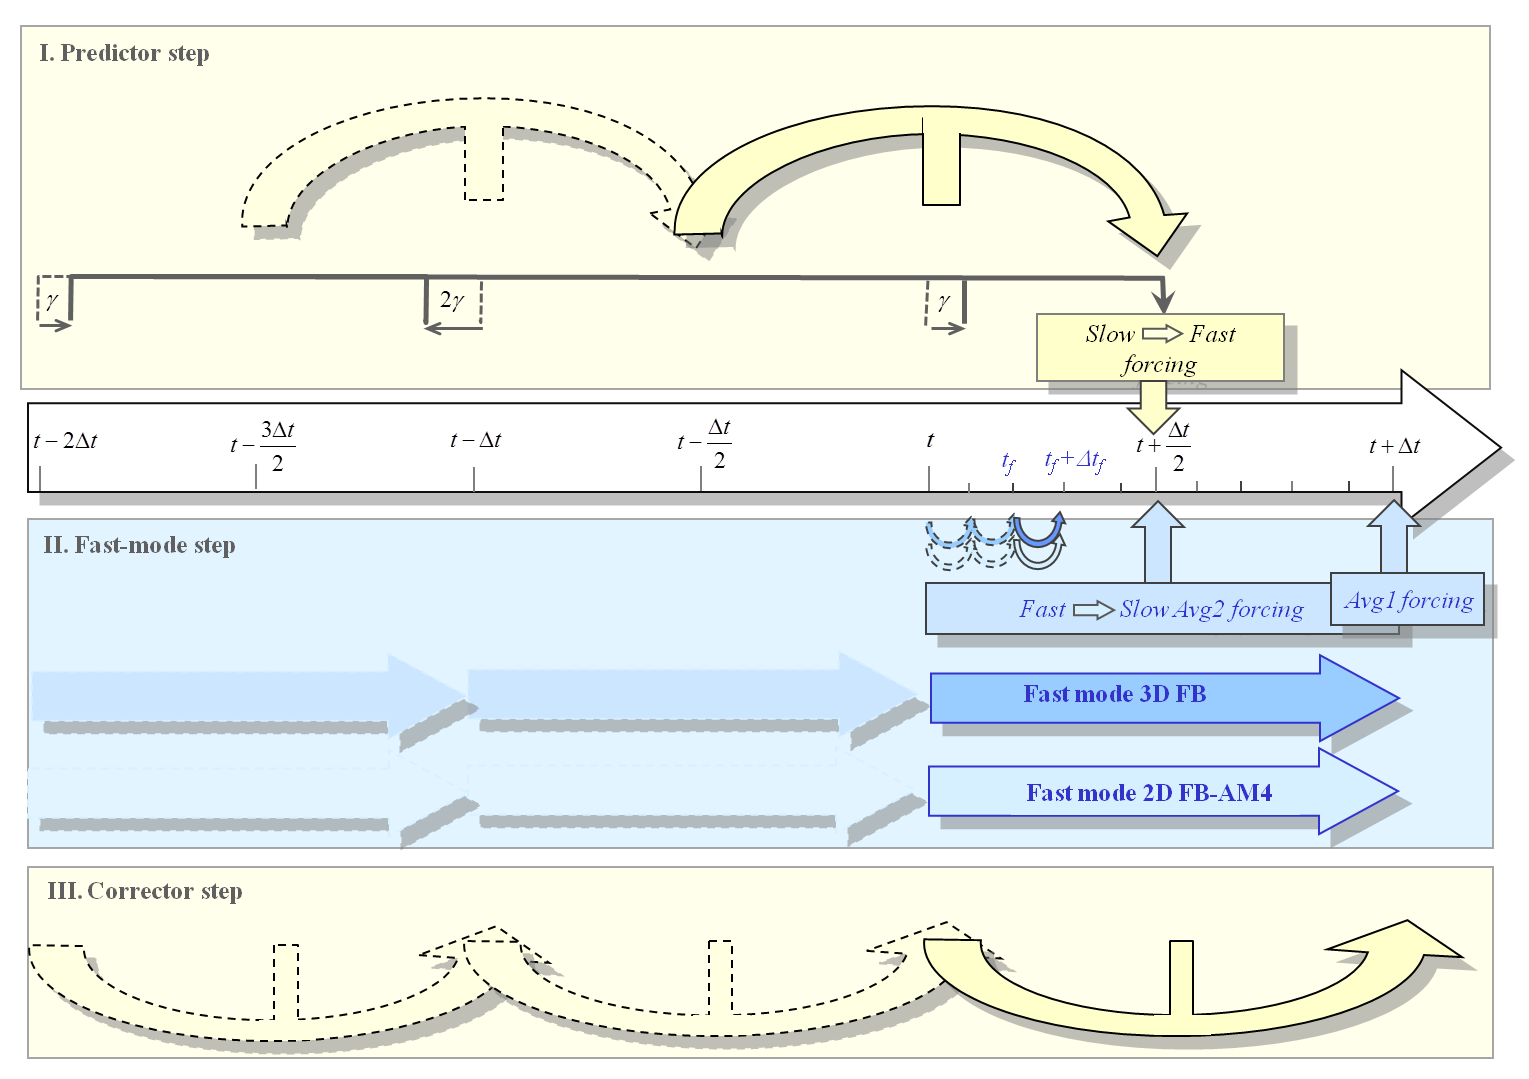
\includegraphics[width=1\linewidth]{CHAP2/Model_TS.png}
		\caption{}
	\end{subfigure}
\caption{ \textit{time-splitting and time-stepping of CROCO model with its non-hydrostatic, compressible (NBQ) kernel. Yellow (blue) background color: slow (fast) kernel. }}
	\label{ModelTS}
\end{figure}
%
\begin{table}
\begin{subequations}
\label{TimeSplit}
\begin{alignat}{3}
 \displaystyle
 %%%%%%%%%%%%%%%%%%%%%%%%%%%%%%%%%%%%%%%%%%%%%%%%%%%%%%%%%%%%%
 &\nonumber \textbf{I.a Time-interpolation: } t_s-\frac{\Delta t_s}{2}\\[0mm]
 %%%%%%%%%%%%%%%%%%%%%%%%%%%%%%%%%%%%%%%%%%%%%%%%%%%%%%%%%%%%%
 \label{TimeSplitIa1}
 &\quad[\Theta] ^{n-\frac{1}{2}}=\alpha_{n-1}\Theta_s^{n-1}
 +\alpha_{n}\Theta^{n}\\[3mm]
 %%%%%%%%%%%%%%%%%%%%%%%%%%%%%%%%%%%%%%%%%%%%%%%%%%%%%%%%%%%%%
 &\nonumber \textbf{I.b Predictor step: } t_s+\frac{\Delta t_s}{2}\\[0mm]
 %%%%%%%%%%%%%%%%%%%%%%%%%%%%%%%%%%%%%%%%%%%%%%%%%%%%%%%%%%%%%
 \label{TimeSplitIb1}
 &\quad\rho h_s\mathbf{v}_s^{n+\frac{1}{2}}=
 [\rho h_s\mathbf{v}_s]^{n-\frac{1}{2}}
 +\Delta t_s\left(\Lambda_{s,v}^{n}+<\Lambda_{f,v}>^n\right)\\[3mm]
 %
 \label{TimeSplitIb2}
 &\quad\rho h_s(\theta_s,\ S_s)^{n+\frac{1}{2}}=
 \rho h_s[\theta_s,\ S_s]^{n-\frac{1}{2}}
 +\Delta t_s\Lambda_{s,(\theta,S)}^{n}\\[3mm]
 %
 \label{TimeSplitIb3}
 &\quad\rho_s^{n+\frac{1}{2}}=\rho_{eos}\left(\theta_s^{n+\frac{1}{2}},\ S_s^{n+\frac{1}{2}},\ z_s^{n+\frac{1}{2}}\right)\\[3mm]
 %
 \label{TimeSplitIb4}
 &\quad\partial_s\omega_s^{n+\frac{1}{2}}=-\partial_t\rho h_s^{n+\frac{1}{2}}
 +\mathbf{\nabla}\cdot\rho h_s \mathbf{u}_s^{n+\frac{1}{2}}\\[3mm]
 %%%%%%%%%%%%%%%%%%%%%%%%%%%%%%%%%%%%%%%%%%%%%%%%%%%%%%%%%%%%%
 &\nonumber \textbf{I.c AB3-extrapolation: } t_s+\frac{\Delta t_s}{2}\\[0mm]
 %%%%%%%%%%%%%%%%%%%%%%%%%%%%%%%%%%%%%%%%%%%%%%%%%%%%%%%%%%%%%
 \label{TimeSplitIc1}
 &\quad[[\Psi_s]]^{n+\frac{1}{2}}=
  \beta_{n-2}\Psi_s^{n-2}
 +\beta_{n-1}\Psi_s^{n-1}
 +\beta_{n}\Psi_s^{n}\\[3mm]
 %%%%%%%%%%%%%%%%%%%%%%%%%%%%%%%%%%%%%%%%%%%%%%%%%%%%%%%%%%%%%
 &\nonumber \textbf{II. Fast-mode steps: } t_f\in(t_s,\ t_s+\Delta t_s] \textit{ or } m\in[0,\ N_f)_\mathcal{N}\\[2mm]
 %%%%%%%%%%%%%%%%%%%%%%%%%%%%%%%%%%%%%%%%%%%%%%%%%%%%%%%%%%%%%
 \label{TimeSplitIIa}
 &\quad\zeta_f^{m+1}=\zeta_f^{m}+\Delta t_f\left(
  w_{surf}^{m}-\mathbf{u}_{surf}^{m}.\mathbf{\nabla}\zeta^{m}\right)\\[3mm]
 %
 \label{TimeSplitIIb}
 &\quad\rho h u_f^{m+1}=
 \rho h u_f^{m}
 +\Delta t_f\left(
  [[\Lambda_{s,u}]]^{n+\frac{1}{2}}
 -[[\overline{\Lambda_{s,u}}]]^{n+\frac{1}{2}}
 +\Lambda_{f,u}^{m}
% +\overline{\overline{\Lambda_{f,u}}}^{\ m}
 +\overline{\overline{\Lambda_{f,u}}}^{\ m}
 +\overline{\overline{\Lambda_{f,-\mathbf{\nabla}\zeta}}}^{\ m+1}
 \right)\\[3mm]
 %
 \label{TimeSplitIIc}
 &\quad\overline{\overline{\rho h U}}_f^{\ m+1}=
 \overline{\overline{\rho h U}}_f^{\ m}
 +\Delta t_f\left(
 %[[\overline{\Lambda_{s,u}}]]^{n+\frac{1}{2}}+
 \overline{\Lambda_{f,u}^{m}}
 +\overline{\overline{\Lambda_{f,u}}}^{\ m}
 +\overline{\overline{\Lambda_{f,-\mathbf{\nabla}\zeta}}}^{\ m+1}
 \right)\\[0mm]
 %
 \label{TimeSplitIId}
 &\quad\rho h w_f^{m+1}=
 \rho h w_f^{m}
 +\Delta t_f\left([[\Lambda_{s,w}]]^{n+\frac{1}{2}}
 +\Lambda_{f,w}^{m+1*}\right)\\[0mm]
 %
 \label{TimeSplitIIe}
 &\quad\rho h_f^{m+1}=\rho h_f^{m}
 -\Delta t_f\left(
 [[\partial_t\rho h_s]]^{n+\frac{1}{2}}
 +\mathbf{\nabla}\cdot\{\rho h \mathbf{v}\}_f^{m+1}
 \right)\\[0mm]
 %
 \label{TimeSplitIIh}
 &\quad \textit{Last\ fast\ time-step ($m=N_f-1$):}\ \bar{\rho}\zeta_s^{n+1}
 =\bar{\rho}(H+\zeta_f)^{m}
 -\bar{\rho}H_s^{m+1}
 -\Delta t_f\mathbf{\nabla}\cdot\overline{\overline{\rho h\mathbf{u}}}^{\ m+1}\\[3mm]
 %
 \label{TimeSplitIIg}
 &\quad \textit{Update\ grid:}\ \rho h_f^{m+1},\ z_f^{m+1}\\[3mm]
 %
 %%%%%%%%%%%%%%%%%%%%%%%%%%%%%%%%%%%%%%%%%%%%%%%%%%%%%%%%%%%%%
 &\nonumber \textbf{III.a Filtering: } t_s+\Delta t_s\ \textit{and}\ t_s+\frac{\Delta t_s}{2}\\[0mm]
 %%%%%%%%%%%%%%%%%%%%%%%%%%%%%%%%%%%%%%%%%%%%%%%%%%%%%%%%%%%%%
 \label{TimeSplitIIIa1}
 &\quad<\Phi_f>^{n+1}=\Phi_f^{m=n+1}\\[0mm]
 \label{TimeSplitIIIa2}
 &\quad\ll\Phi_f\gg^{n+\frac{1}{2}}=\frac{1}{N_f}\sum_{m=1}^{N_f}\Phi_f^{m}\\[3mm]
 %%%%%%%%%%%%%%%%%%%%%%%%%%%%%%%%%%%%%%%%%%%%%%%%%%%%%%%%%%%%%
 &\nonumber \textbf{III.b Corrector step: } t_s+\Delta t_s\\[0mm]
 %%%%%%%%%%%%%%%%%%%%%%%%%%%%%%%%%%%%%%%%%%%%%%%%%%%%%%%%%%%%%
 %
 \label{TimeSplitIIIb1}
 &\quad\rho h_s\mathbf{v}_s^{n+1}=
 \rho h_s\mathbf{v}_s^{n}
 +\Delta t_s\left(\Lambda_s^{n+\frac{1}{2}*}
 +\ll\Lambda_f\gg^{n+\frac{1}{2}}\right)\\[0mm]
 %
 \label{TimeSplitIIIb2}
 &\quad\partial_s\omega_s^{n+1}=
 -\partial_{t\ }\rho h_s^{n+1}
 +\mathbf{\nabla}\cdot\rho h_s \mathbf{u}_s^{\ n+1}
 -\overline{\mathbf{\nabla}\cdot\rho h_s \mathbf{u}_s}^{\ n+1}
 -\overline{<\mathbf{\nabla}\cdot\rho h_s \mathbf{u}_s>}^{\ n+1}\\[3mm]
 %
 \label{TimeSplitIIIb3}
 &\quad\rho h_s(\theta_s,\ S_s)^{n+1}=
 \rho h_s(\theta_s,\ S_s)^{n}
 +\Delta t_s\Lambda_{s,(\theta,S)}^{n+\frac{1}{2}*}\\[0mm]
 %
 \label{TimeSplitIIIb4}
 &\quad\rho_s^{n+1}=\rho_{eos}\left(\theta_s^{n+1},\ S_s^{n+1},\ z_s^{n+1}\right)\\[0mm]
 %
 \label{TimeSplitIIIb5}
 &\quad\rho h_s\mathbf{u}_s^{n+1}=\rho h_s\mathbf{u}_s^{n+1}
 -\overline{\rho h_s\mathbf{u}_s}^{\ n+1}
 +\overline{\rho h\mathbf{u}_f}^{\ m=N_f-1}
 %%%%%%%%%%%%%%%%%%%%%%%%%%%%%%%%%%%%%%%%%%%%%%%%%%%%%%%%%%%%%
\end{alignat}
\end{subequations}
\end{table}
Predictor (I), fast-kernel Forward-Backward (II) and Corrector (III) steps are shown in horizontal color bands (yellow for the slow kernel, blue for the fast kernel) on figure \ref{ModelTS}. After time-interpolating slow-kernel variables to time-step $t_s-\Delta t_s/2$ (step I.a, notation $[.]$), the slow kernel is advanced from $t_s-\Delta t_s/2$ to $t_s+\Delta t_s/2$ with a centered, leap-frog-like, time-stepping (step I.b). Then, to prepare the integration of the fast kernel, the slow-kernel RHS is extrapolated to $t_s+\Delta t_s/2$ based on an AB3 scheme using its previous evaluations at $t_s-2\Delta t_s$, $t_s-\Delta t_s$ and $t_s$ (step I.c, notation $[[.]]$). The fast kernel can in turn be advanced from $t_s$ to $t_s+\Delta t_s$ using a forward-backward time-stepping (step II) with time-step $\Delta t_f$ satisfying  $N_f=\Delta t_s/\Delta t_f\in\mathcal{N}$. The vertical grid is updated at each fast time-step \ref{TimeSplitIIg} but slow-kernel components of the RHS remain constant during the fast-kernel integration. At the last fast time-step, surface elevation displacement for the slow kernel can be recomputed to ensure perfect numerical coherence between the surface kinematic relation and depth-integrated mass conservation (\noparref{TimeSplitIIa} and \noparref{TimeSplitIIh}). 
%The barotropic-like, depth-independent component is also integrated with the same time-step $\Delta t_f$ with a forward-backward scheme as in \cite{shchepetkin_regional_2005}. 
A major difference with the hydrostatic time-splitting is that the surface elevation displacement is given by the kinematic condition \ref{TimeSplitIIa} and not by the depth-integral of the mass conservation equation. Once the fast-kernel RHS and variables have been filtered both at $t_s+\Delta t_s$ and $t_s+\Delta t_s/2$ (step III.a, notations $<.>$ and $\ll.\gg$), the slow kernel is finally advanced from $t$ to  $t_s+\Delta t_s$ during the leap-frog-like Corrector step (III.b).\\
Note that the 2D depth-average, barotropic-like, horizontal momentum equations \ref{TimeSplitIIc} are advanced in the same way as in \cite{shchepetkin_regional_2005}. The result of this 2D integration is indeed used to correct both the horizontal momentum itself and the RHS of the horizontal momentum equation at Corrector step. It can also be used to require a perfect coherence of the surface elevation displacement and the depth-average transport (at machine precision) during slow-mode integration. 

\subsection{Sub-grid mixing and parametrisation}

\subsubsection{LES,RANS,etc numerical models}
Numerical models are discretized and have a treshold resolution under which phyisical pehomenons cannot be represented explicitely. Particularly, diffusion and ... processes,  among other parametrisations of processes like surface exchanges, radiation that occur at molecular or submolecular scales. Diffusion and dissipation are molecular in nature as a , energy flux, but more broadly speaking, dissipation is the transfer of energy from great scales to small scales. In a stratified fluid, this dissipation is accompagnied by mixing , ie a lewoering of potential energy, or more accurately and explained i paragraph ..., of the background potential energy.

Broadly for oceanic (or more generally geophyisic?) models classification on DNS, LES, and RANS. DNS has molecular dissipation


For the discussions simply coining as LES is not sufficient but need to precise LES in regard to which phenomenon. For exemplein chapoter ... of this manuscript, coined LES because primary instabilities of the flow. However, the primary instabilities that are known to exist at upper and lower boundaries of teh water column are not represented and are parametrized, so in regard to the dissipation those process not LES. 



To this considerations, one must also not forget that the discretisation itself introduces numerical dissipation unless using centered schemes (computationnally impossible).

\subsubsection{Two parametrisation in this manuscript}
Present here two of the parametrisations available in CROCO that are used inthis manuscript.

\paragraph{Smagorinsky}


\paragraph{GLS k-$\epsilon$}






















\section{Annexe : formulaire coordinate transformation}
%%%%%%%%%%%%%%%%%%%%%%%%%%%%%%%%%%%%%%%%%%%%%%%%%%%%%%%%%%%%%%%%%%%%%%%%%%%%%
\subsubsection{Coordinate transformation}
\label{annexe_coordS}
%%%%%%%%%%%%%%%%%%%%%%%%%%%%%%%%%%%%%%%%%%%%%%%%%%%%%%%%%%%%%%%%%%%%%%%%%%%%%
The transformation matrix of the generalized coordinate transformation is:
\begin{equation}
    \displaystyle
    \Lambda^z_s=
    \begin{pmatrix}
    1 & 0 & 0 & 0 \\
    0 & 1 & 0 & 0 \\
    0 & 0 & 1 & 0 \\
    \frac{\partial z}{\partial t} & \frac{\partial z}{\partial x}
    & \frac{\partial z}{\partial y} & h=\frac{\partial z}{\partial s}
    \end{pmatrix}
\end{equation}
The inverse transformation is given by:
\begin{equation}
    \displaystyle
    \Lambda_z^s=
    \begin{pmatrix}
    1 & 0 & 0 & 0 \\
    0 & 1 & 0 & 0 \\
    0 & 0 & 1 & 0 \\
    \frac{\partial s}{\partial t} & \frac{\partial s}{\partial x}
    & \frac{\partial s}{\partial y} & \frac{\partial s}{\partial z}
    \end{pmatrix}
\end{equation}

The Jacobian of the transformation $J=det(\Lambda^z_s)$ is the (specific) thickness:
\begin{equation}
 \displaystyle
 J=h=\frac{\partial z}{\partial s}=\frac{\partial z}{\partial s}\bigg\vert_{xyt}
\end{equation}
\cite{griffies_fundamentals_2004} further define the infinitesimal  thickness for modelling developments:
\begin{equation}
 \displaystyle
 \delta h=\frac{\partial z}{\partial s} \delta s
\end{equation}

%%%%%%%%%%%%%%%%%%%%%%%%%%%%%%%%%%%%%%%%%%%%%%%%%%%%%%%%%%%%%%%%%%%%%%%%%%%%%
\subsubsection{Formula and identities(idem annexe?)}
%%%%%%%%%%%%%%%%%%%%%%%%%%%%%%%%%%%%%%%%%%%%%%%%%%%%%%%%%%%%%%%%%%%%%%%%%%%%%
Coordinate transformations are given by:
\begin{subequations}
  \begin{alignat}{2}
  \displaystyle 
  &\frac{\partial A}{\partial t}\bigg\rvert_{xz} &&=
   \frac{\partial A}{\partial t}\bigg\rvert_{xs}
  - \frac{1}{h} \frac{\partial A}{\partial s}\bigg\rvert_{tx}
  \frac{\partial z}{\partial t}\bigg\rvert_{xs}\\
  &\frac{\partial A}{\partial x}\bigg\rvert_{tz} &&=
   \frac{\partial A}{\partial x}\bigg\rvert_{ts}
  - \frac{1}{h} \frac{\partial A}{\partial s}\bigg\rvert_{tx}
  \frac{\partial z}{\partial x}\bigg\rvert_{ts}\\
  &\frac{\partial A}{\partial z}\bigg\rvert_{tx} &&=
   \frac{1}{h}
   \frac{\partial A}{\partial s}\bigg\rvert_{tx}
  \end{alignat}
\end{subequations}
Material derivatives satisfy:
\begin{subequations}
  \begin{alignat}{2}
  \displaystyle 
  & \frac{d}{dt} &&=\frac{\partial}{\partial t}\bigg\vert_z
  + \mathbf{u}.\mathbf{\nabla}_z
  + w\frac{\partial }{\partial z}\\
  & &&=\frac{\partial}{\partial t}\bigg\vert_s
  + \mathbf{u}.\mathbf{\nabla}_s
  + \dot{s}\frac{\partial}{\partial s}
  \end{alignat}
\end{subequations}
which leads to:
\begin{subequations}
  \begin{alignat}{2}
  \displaystyle 
  & \dot{z} &&=\frac{dz}{dt}\bigg\vert_s=\frac{\partial z}{\partial t}\bigg\vert_s
  + \mathbf{u}.\mathbf{\nabla}_s z
  + \dot{s}\frac{\partial z}{\partial s}\\
  & \dot{s} &&=\frac{ds}{dt}\bigg\vert_z=\frac{\partial s}{\partial t}\bigg\vert_z
  + \mathbf{u}.\mathbf{\nabla}_z s
  + w\frac{\partial s}{\partial z}
  \end{alignat}
\end{subequations}
Using the identities:
\begin{subequations}
  \begin{alignat}{2}
  \displaystyle
  &\frac{\partial s}{\partial t}\bigg\vert_z &&=
  \left(\frac{\partial t}{\partial s}\bigg\vert_z\right)^{-1}\\
  &\frac{\partial s}{\partial x}\bigg\vert_z &&=
  \left(\frac{\partial x}{\partial s}\bigg\vert_z\right)^{-1}\\
  &\frac{\partial s}{\partial y}\bigg\vert_z &&=
  \left(\frac{\partial y}{\partial s}\bigg\vert_z\right)^{-1}\\
  &\frac{\partial s}{\partial z}\bigg\vert_x &&=
  \left(\frac{\partial z}{\partial s}\bigg\vert_x\right)^{-1}
  \end{alignat}
\end{subequations}
several relations are obtained from the triple product rule:
Coordinate transformations are given by:
\begin{subequations}
  \begin{alignat}{2}
  \displaystyle
  &\frac{\partial z}{\partial t}\bigg\vert_s &&=
  -\frac{\partial s}{\partial t}\bigg\vert_z\frac{\partial z}{\partial s}\bigg\vert_s\\
  &\frac{\partial z}{\partial x}\bigg\vert_s &&=
  -\frac{\partial s}{\partial x}\bigg\vert_z\frac{\partial z}{\partial s}\bigg\vert_s\\
  &\frac{\partial z}{\partial y}\bigg\vert_s &&=
  -\frac{\partial s}{\partial y}\bigg\vert_z\frac{\partial z}{\partial s}\bigg\vert_s\\
  \end{alignat}
\end{subequations}

%%%%%%%%%%%%%%%%%%%%%%%%%%%%%%%%%%%%%%%%%%%%%%%%%%%%%%%%%%%%%%%%%%%%%%%%%%%%%
\subsubsection{Local orthonormal coordinates (annexe?plus tard...)}
%%%%%%%%%%%%%%%%%%%%%%%%%%%%%%%%%%%%%%%%%%%%%%%%%%%%%%%%%%%%%%%%%%%%%%%%%%%%%
\cite{griffies_fundamentals_2004} further defines in his chapter (6.4) a system of orthonormal coordinates:
\begin{subequations}
  \begin{alignat}{2}
  \displaystyle 
  &\mathbf{e}_{x^*} &&=\frac{\mathbf{y}\wedge{\mathbf{\nabla}s}}
  {\norm{\mathbf{y}\wedge{\mathbf{\nabla}s}}}\\
  &\mathbf{e}_{y^*} &&=\mathbf{e}_s\wedge{\mathbf{e}_{x^*}}\\
  &\mathbf{e}_s &&=\frac{\mathbf{\nabla}s}{\norm{\mathbf{\nabla}s}}
  \end{alignat}
\end{subequations}
In this particular case ($\mathbf{e}_s.\mathbf{z}$ has a unique signe, the basis vectors can be rewritten:
\begin{subequations}
  \begin{alignat}{2}
  \displaystyle 
  &\mathbf{e}_{x^*} &&=\frac{\mathbf{x}+S_x\mathbf{z}}{\sqrt{1+S_x^2}}\\
  &\mathbf{e}_{y^*} &&=\frac{-S_xS_y\mathbf{x}+(1+S_x^2)\mathbf{y}+S_y\mathbf{z}}{\sqrt{1+S^2)(1+S_x^2)}}\\
  &\mathbf{e}_s &&=\frac{(-\mathbf{S},1)}{\sqrt{1+S^2}}
  \end{alignat}
\end{subequations}
The s-coordinate transformation is a rotation and:
\begin{equation}
   \displaystyle
   \mathbf{e}_{x^*y^*s}=\Lambda_{s}^{z}\mathbf{e}_{xyz}
\end{equation}
Note in particular the definition of the slope $\mathbf{S}$ and its norm $S=\norm{\mathbf{S}}$ used to rewrite the orthonormal basis:
\begin{equation}
   \displaystyle
   \mathbf{S}=\mathbf{\nabla}_s z=
   -\frac{\partial z}{\partial s}\mathbf{\nabla}_z s=\left( S_x,\ S_y,\ 0 \right)
\end{equation}
where $\mathbf{\nabla}_s z$ is "the horizontal gradient of the height of a fluid parcel as taken along surfaces of constant generalized vertical coordinate s" \citep{griffies_fundamentals_2004}.\\
\textbf{Caution:} this orthonormal basis is not used to project the equations of the model. S-coordinates are "only" used as a change of variable whereas equations and vector quantities remain written in the original Cartesian or spherical basis. The present s-coordinate orthonormal basis is presented here to be latter used in the computation of fluxes through s-surfaces.






%%%%%%%%%%%%%%%%%%%%%%%%%%%%%%%%%%%%%%%%%%%%%%%%%%%%%%%%%%%%%%%%%%%%%%%%%%%%%
\section{Annexe : Reynolds Theorem}
\label{annexe_reynolds}
%%%%%%%%%%%%%%%%%%%%%%%%%%%%%%%%%%%%%%%%%%%%%%%%%%%%%%%%%%%%%%%%%%%%%%%%%%%%%
\subsubsection{Flux through a surface}
%%%%%%%%%%%%%%%%%%%%%%%%%%%%%%%%%%%%%%%%%%%%%%%%%%%%%%%%%%%%%%%%%%%%%%%%%%%%%
Based on \citep{delhaye_thermohydraulique_2008}, let $\mathbf{v}_{\Sigma}$ be the velocity of a material surface in the fluid:
\begin{equation}
	\displaystyle
	\mathbf{v}_{\Sigma}=\frac{\partial \mathbf{x}}{\partial t}\bigg\rvert _{\Sigma}
\end{equation}
with $\mathbf{x}$ the position of the current point where the velocity is computed. This velocity is undetermined  since the tangential component is itself undetermined. Only its normal component $(\mathbf{n}_{\Sigma}.\mathbf{v}_{\Sigma})$ can be computed and isolated. This component is different from the vertical component of $\mathbf{v}_{\Sigma}$ of equation \ref{eq_vertvelcomp}.\\

Demonstrations and further expressions of the normal component can be found in \citet{griffies_fundamentals_2004}, \citet{griffies_elements_2012} and \citet{delhaye_thermohydraulique_2008}.
\begin{subequations}
  \begin{alignat}{2}
  \displaystyle 
  & \frac{\partial z}{\partial t}\bigg\vert_s &&=
  \frac{\partial s}{\partial t}\bigg\vert_z
  \frac{\partial z}{\partial s}\bigg\vert_t\\
  & &&=h\norm{\mathbf{\nabla}s}\mathbf{n}_{\Sigma}.
  \mathbf{v}_{\Sigma}
  \end{alignat}
\end{subequations}
Metric tensor formulations lead to:
\begin{subequations}
  \begin{alignat}{2}
 & dS_{\Sigma} &&= h\norm{\mathbf{\nabla}s} dS\\
 & h dS &&=\mathbf{n}_{\Sigma}.\mathbf{v}_{\Sigma}dS_{\Sigma}
  \end{alignat}
\end{subequations}
%See bellow how this formula is used to write Leibniz rule...

\subsubsection{Formulations of the Reynolds Transport Theorem (\& Leibniz Rule)}
\paragraph{Demonstration}
The difficulty to compute:
\begin{equation}
 \displaystyle
 \frac{d}{dt} \iiint_{\mathcal{V}_M(t)} \rho A d\tau
\end{equation}
is due to the fact that for a general time-varying volume $\mathcal{V}(t)$ the differentiation cannot be taken through the internal sign. To do so, we can however consider a change of coordinates to volume-attached coordinates \citep{hirasaki_chapter_2021}. Let $\mathcal{J}$ be the Jacobian (determinant of the Jacobian matrix) of the change of variables from Cartesian coordinates $(\mathbf{x},t)$ to volume varying coordinates $(\boldsymbol{\xi},t)$. Integrating volume is $\mathcal{V}(t)=\mathcal{V}_{\xi}=\mathcal{V}_{\xi}(t)$.\\
Kinematic evolution of material particulate ("dilation kinematic theorem") is then nothing but Reynolds'transport theorem (which is equivalent to Leibniz derivation rule to 3D volumes) \citep{hirasaki_chapter_2021}. Caution: the demonstration given in \citep{hirasaki_chapter_2021} is for a material volume $\mathcal{V}_M$. As the demonstration is kinematic, it is generalized here to a general volume moving thought the fluid flow $(\mathcal{V}(t))$. This problem is dealt with in \cite{web_course_web_2021} (and further references are given in there).\\
As a consequence for a general volume $\mathcal{V}(t)$ moving at a 3D velocity $  \mathbf{v}_{\Sigma}$:
\begin{equation}
 \displaystyle
 \frac{dJ}{dt}=J \mathbf{\nabla}.\mathbf{v}_{\Sigma}
\end{equation}
which is reminiscent of the kinematic evolution of the specific volume of a fluid particle:
\begin{equation}
 \displaystyle
 \frac{d\tau}{dt}=\tau \mathbf{\nabla}.\mathbf{v}
\end{equation}
sometime written:
\begin{equation}
 \displaystyle
 \frac{d\delta\tau}{dt}=\delta\tau \mathbf{\nabla}.\mathbf{v}
\end{equation}
which is noting but the continuity equation written for the specific volume.

With the natural change of variable, the derivation can enter the integral sign and:
\begin{subequations}
  \begin{alignat}{2}
  \displaystyle 
  & \frac{d}{dt} \iiint_{\mathcal{V}(t)} \rho A d\tau &&=
  \frac{D}{Dt} \iiint_{\mathcal{V}(t)} \rho A d\tau\\
  & &&= \frac{D}{Dt} \iiint_{\mathcal{V}(t)} \rho A d\mathbf{x}\\
  & &&=\frac{D}{Dt} \iiint_{\mathcal{V}_{\xi}} \rho A J d\boldsymbol{\xi}\\
  & &&=\iiint_{\mathcal{V}_{\xi}} \frac{D\rho A}{Dt}  J d\boldsymbol{\xi}
  +\iiint_{\mathcal{V}_{\xi}} \rho A \frac{DJ}{Dt} d\boldsymbol{\xi}\\
  & &&=\iiint_{\mathcal{V}_{\xi}} \frac{D\rho A}{Dt}  J d\boldsymbol{\xi}
  +\iiint_{\mathcal{V}_{\xi}} \rho A \mathbf{\nabla}. \mathbf{v}_{\Sigma}\ J d\boldsymbol{\xi}
  \end{alignat}
\end{subequations}
Following \cite{truesdell_classical_1960}, a more general formulation can thus be recovered for a time-dependant volume $\mathcal{V}(t)$ moving with a velocity $\mathbf{v}_{\Sigma}$:
\begin{subequations}
  \begin{alignat}{2}
  \displaystyle 
  &  \frac{d}{dt} \iiint_{\mathcal{V}(t)} \rho A d\tau && =
  \iiint_{\mathcal{V}(t)} \frac{D\rho A}{Dt}  d\boldsymbol{x}
  +\iiint_{\mathcal{V}(t)} \rho A \mathbf{\nabla}.\mathbf{v}_{\Sigma}\ d\mathbf{x}\\
 & && =
  \iiint_{\mathcal{V}(t)} \frac{\partial \rho A}{\partial t}\bigg\rvert_{xz} d\tau
  %+ \varoiint_{\mathcal{V}(t)}\rho A \mathbf{v}.\mathbf{S}\\
  + \oiint_{\mathcal{S}(t)}\rho A   \mathbf{v}_{\Sigma}.\mathbf{n}_{\Sigma}dS_{Sigma}
  \end{alignat}
\end{subequations}
where:
\begin{equation}
 \displaystyle
 \frac{D\bullet}{Dt}=\frac{\partial \bullet}{\partial t}\bigg\vert_{\boldsymbol{\xi}}
 +  \mathbf{v}_{\Sigma}.\mathbf{\nabla}_{t,\boldsymbol{\xi}}\bullet
\end{equation}
This is the generalized (Reynolds) transport theorem or the generalized Leibnitz theorem. Caution: the derivative $D/Dt$ is associated to $  \mathbf{v}_{\Sigma}$.

\paragraph{Closed time-dependent volume $\mathcal{V}(t)$}
Several formulations of this kinematic theorem can be given:
\begin{subequations}
  \begin{alignat}{2}
  \displaystyle 
  & \frac{d}{dt} \iiint_{\mathcal{V}(t)} \rho A d\tau &&=
  \iiint_{\mathcal{V}(t)} \frac{\partial \rho A}{\partial t}\bigg\rvert_{xz} d\tau
  %+ \varoiint_{\mathcal{V}(t)}\rho A \mathbf{v}.\mathbf{S}\\
  + \oiint_{\mathcal{V}(t)}\rho A   \mathbf{v}_{\Sigma}.d\mathbf{S}\\\\
  % Line 2:
  &  &&= \iiint_{\mathcal{V}(t)} \left(\frac{\partial \rho A}{\partial t}\bigg\rvert_{xz}
  +\mathbf{\nabla}.(\rho A   \mathbf{v}_{\Sigma}) \right) d\tau\\
  % Line 3:
  &  &&= \iiint_{\mathcal{V}(t)} \left(\rho \frac{\partial A}{\partial t}\bigg\rvert_{xz}
  +A \frac{ \partial \rho }{\partial t}\bigg\rvert_{xz}
  +\rho   \mathbf{v}_{\Sigma}.\mathbf{\nabla}A 
  +A\mathbf{\nabla}.(\rho   \mathbf{v}_{\Sigma}) \right) d\tau\\
  % Line 4:
  & &&=\iiint_{\mathcal{V}(t)} \rho \frac{DA}{Dt}  d\tau 
  +\iiint_{\mathcal{V}(t)} A \left( \frac{\partial \rho}{\partial t} \bigg\rvert_{xz}
  +\mathbf{\nabla}.(\rho  \mathbf{v}_{\Sigma})\right) \ d\tau
  \end{alignat}
\end{subequations}
This can also be written:
\begin{subequations}
  \begin{alignat}{2}
  \displaystyle 
  & \frac{d}{dt} \iiint_{\mathcal{V}(t)} \rho A d\tau &&=
   \iiint_{\mathcal{V}(t)} \left(\rho \frac{\partial A}{\partial t}\bigg\rvert_{xz}
  +A \frac{ \partial \rho }{\partial t}\bigg\rvert_{xz}
  +\rho   \mathbf{v}_{\Sigma}.\mathbf{\nabla}A 
  +A   \mathbf{v}_{\Sigma}.\mathbf{\nabla}\rho
  +A\rho\mathbf{\nabla}.  \mathbf{v}_{\Sigma} \right) d\tau\\
  % Line 2:
  & &&=\iiint_{\mathcal{V}(t)} \rho \frac{DA}{Dt}  d\tau 
  +\iiint_{\mathcal{V}(t)} A \frac{D \rho}{D t} d\tau
  + \iiint_{\mathcal{V}(t)} \rho A\mathbf{\nabla}.  \mathbf{v}_{\Sigma} d\tau
  \end{alignat}
\end{subequations}
or alternatively:
\begin{subequations}
  \begin{alignat}{2}
  \displaystyle 
  & \frac{d}{dt} \iiint_{\mathcal{V}(t)} \rho A d\tau &&
  =\iiint_{\mathcal{V}(t)} \rho \frac{dA}{dt}  d\tau 
  +\iiint_{\mathcal{V}(t)} \left(A \frac{d \rho}{dt} 
  +\mathbf{\nabla}.\left[ \rho A(  \mathbf{v}_{\Sigma}-\mathbf{v})\right]
  +\rho A \mathbf{\nabla}.\mathbf{v} \right) d\tau\\
  & &&
  =\iiint_{\mathcal{V}(t)} \rho \frac{dA}{dt}  d\tau 
  + \iiint_{\mathcal{V}(t)}\mathbf{\nabla}.\left[ \rho A(  \mathbf{v}_{\Sigma}-\mathbf{v})\right]d\tau
    \end{alignat}
\end{subequations}
where $  \mathbf{v}_{\Sigma}$ is defined as the velocity of the closed surface of $\mathcal{V}(t)$ and is more generally the 3D displacement velocity of the volume $\mathcal{V}(t)$.\\
 Caution: this has nothing to do with the velocity of the fluid in this volume except in the following particular case when considering a material volume, i.e. in the Lagrangian approach.
These general formulations and demonstrations are useful in s-coordinates.

\subsubsection{Material volume $\mathcal{V}_M(t)$ (kinematics \& dynamics)}
\paragraph{Formulation of the transport theorem}
A material volume $\mathcal{V}_M(t)$ is defined as a volume containing exactly the same fluid particles as time goes on.
Simplifications to obtain the simple expression of the integral variations in the case of a moving material volume are based on the use of the continuity equation or conservation of mass. \\
As the control volume is advected by mean flow (Lagrangian approach), $  \mathbf{v}_{\Sigma}=\mathbf{v}$ :
\begin{equation}
  \displaystyle 
   \frac{d}{dt} \iiint_{\mathcal{V}_M(t)} \rho A d\tau =
  \iiint_{\mathcal{V}_M(t)} \rho \frac{dA}{dt}  d\tau 
  +\iiint_{\mathcal{V}_M(t)} A \frac{d \rho}{dt} d\tau
  +\iiint_{\mathcal{V}_M(t)} \rho A\mathbf{\nabla}.\mathbf{v} d\tau
\end{equation}
and thus:
\begin{subequations}
  \begin{alignat}{2}
  \displaystyle 
  & \frac{d}{dt} \iiint_{\mathcal{V}_M(t)} \rho A d\tau &&= \iiint_{\mathcal{V_M}(t)} \rho \frac{dA}{dt}  d\tau 
  +\iiint_{\mathcal{V}_M(t)} A \underbrace{\left( \frac{\partial \rho}{\partial t} \bigg\rvert_{xz}+\mathbf{\nabla}.(\rho\mathbf{v})\right)}_{=0} \ d\tau\\
  & && = \iiint_{\mathcal{V}_M(t)} \rho \frac{dA}{dt}  d\tau 
  \end{alignat}
\end{subequations}
This is a generalization to 3D volume of the Leibniz rule. The time dependency of the integral volume $\mathcal{V}_M(t)$ is for a Lagrangian evolution with time-dependent boundaries. The present formulation is to be used for time-dependent boundaries whatever the velocity $  \mathbf{v}_{\Sigma}$ inside the volume.

\paragraph{Material volume $\mathcal{V}_M(t)$ in Lagrangian material coordinates}
The same exact approach and demonstration can be carried out in the case of a material volume as in the general case.
Let in this case $\mathcal{J}$ be the Jacobian (determinant of the Jacobian matrix) of the change of variables from Cartesian coordinates $(\mathbf{x},t)$ to material coordinates $(\boldsymbol{\xi},t)$. Integrating volume is $\mathcal{V}(t)=\mathcal{V}_{\xi}$.\\
Kinematic evolution of material particle ("dilation kinematic theorem") reads \citep{hirasaki_chapter_2021}:
\begin{equation}
 \displaystyle
 \frac{dJ}{dt}=J \mathbf{\nabla}.\mathbf{v}
\end{equation}
which is reminiscent of the kinematic evolution of a control volume:
\begin{equation}
 \displaystyle
 \frac{d\tau}{dt}=\tau \mathbf{\nabla}.\mathbf{v}
\end{equation}
With this kinematic theorem:
\begin{subequations}
  \begin{alignat}{2}
  \displaystyle 
  & \frac{d}{dt} \iiint_{\mathcal{V}_M(t)} \rho A d\tau &&=
  \frac{d}{dt} \iiint_{\mathcal{V}_M(t)} \rho A d\mathbf{x}\\
  & &&=\frac{d}{dt} \iiint_{\mathcal{V}_{s}} \rho A J d\boldsymbol{\xi}\\
  & &&=\iiint_{\mathcal{V}_{\xi}} \frac{d\rho A}{dt}  J d\boldsymbol{\xi}
  +\iiint_{\mathcal{V}_{\xi}} \rho A \frac{dJ}{dt} d\boldsymbol{\xi}\\
  & &&=\iiint_{\mathcal{V}_{\xi}} \frac{d\rho A}{dt}  J d\boldsymbol{\xi}
  +\iiint_{\mathcal{V}_{\xi}} \rho A \mathbf{\nabla}.\mathbf{v}\ J d\boldsymbol{\xi}
  \end{alignat}
\end{subequations}
This leads finally to:
\begin{subequations}
  \begin{alignat}{2}
  \label{dintdt_s}
  \displaystyle 
  & \frac{d}{dt} \iiint_{\mathcal{V}_M(t)} \rho A d\tau &&=
  \iiint_{\mathcal{V}_{\xi}}\left( \frac{\partial \rho A}{\partial t}   
  +\mathbf{\nabla}.( \rho A \mathbf{v})\right) J d\boldsymbol{\xi} \\
  & && =\iiint_{\mathcal{V}_M(t)} \frac{\partial \rho A}{\partial t}\bigg\rvert_{xz} d\tau
  + \oiint_{\mathcal{V}_M(t)}\rho A \mathbf{v}.d\mathbf{S}
  \end{alignat}
\end{subequations}
Reynolds transport theorem is recovered for a material volume, understood as a volume containing  the same fluid particles. This last relation can be viewed as the difference between the time variation of the extensive variable inside the domaine and the advective flux through the "control" surface matching at time "t" with material volume.

\paragraph{Time-independant "control" volume $\mathcal{V}_0$}
In the particular case when the volume (and thus his surface) is independent of time, then $  \mathbf{v}_{\Sigma}=0$ and as a consequence:
\begin{equation}
 \displaystyle
 	\frac{d}{dt}\iiint_{\mathcal{V}_0} A d\tau = \iiint_{\mathcal{V}_0}\frac{\partial A}{\partial t} d\tau
\end{equation}

\subsection{Formulations based on total derivatives (toward Lagrangian relations...)}
Note that the continuity equation can be written:
\begin{equation}
	\displaystyle
	\frac{d\ \delta \tau}{dt}=\frac{\partial v_{k}}{\partial x_k} \delta\tau= \mathbf{\nabla}.\mathbf{v}\ \delta\tau
\end{equation}

and so for a closed, moving volume $\mathcal{V}(t)$:
\begin{subequations}
  \begin{alignat}{2}
  \displaystyle 
  & \frac{d}{dt} \iiint_{\mathcal{V}(t)} \rho A d\tau &&=  
  \iiint_{\mathcal{V}(t)} \rho \frac{DA}{Dt}  d\tau 
  +\iiint_{\mathcal{V}(t)} A \frac{D(\rho d\tau)}{Dt}\\\\
  & && =  \iiint_{\mathcal{V}(t)} \rho \frac{DA}{Dt}  d\tau 
  + \iiint_{\mathcal{V}(t)} A \frac{D\rho}{Dt} d\tau
  +\iiint_{\mathcal{V}(t)} \rho A \frac{Dd\tau}{Dt} \\
  & && = \iiint_{\mathcal{V}(t)} \rho \frac{DA}{Dt}  d\tau 
  +\iiint_{\mathcal{V}(t)} A \frac{D\rho}{Dt} d\tau
  +\iiint_{\mathcal{V}(t)} \rho A \mathbf{\nabla}.  \mathbf{v}_{\Sigma}\ d\tau \\
  & && = \iiint_{\mathcal{V}(t)} \rho \frac{DA}{Dt}  d\tau 
  \end{alignat}
\end{subequations}
where $D\bullet/Dt=\partial \bullet/\partial t+  \mathbf{v}_{\Sigma}.\mathbf{\nabla}\bullet$. The last simplification is associated to the conservation of mass when written:
\begin{equation}
 \displaystyle
 \frac{D\rho}{Dt}=-\rho\mathbf{\nabla}.  \mathbf{v}_{\Sigma}
\end{equation}
If the volume is now a material volume and is thus advected by the mean flow (Lagrangian approach), $  \mathbf{v}_{\Sigma}=\mathbf{v}_M$ and $D./Dt =d./dt$ :
\begin{subequations}
  \begin{alignat}{2}
  \displaystyle 
  &  \frac{d}{dt} \iiint_{\mathcal{V}_M(t)} \rho A d\tau && = 
  \iiint_{\mathcal{V}_M(t)} \rho \frac{dA}{dt}  d\tau 
  +\iiint_{\mathcal{V}_M(t)} A \frac{d\rho}{dt} d\tau
  +\iiint_{\mathcal{V}_M(t)} \rho A \mathbf{\nabla}.\mathbf{v} d\tau\\
  & && \left[ =\iiint_{\mathcal{V}_M(t)} \rho \frac{dA}{dt}  d\tau 
  +\iiint_{\mathcal{V}_M(t)} A  \underbrace{\left(\frac{\partial \rho}{\partial t} 
  +\underbrace{\mathbf{v}.\mathbf{\nabla}\rho+\rho \mathbf{\nabla}.\mathbf{v} }_{=\mathbf{\nabla}.(\rho\mathbf{v})}\right)}_{=0} d\tau \right]\\
  & && = \iiint_{\mathcal{V}_M(t)} \rho \frac{dA}{dt}  d\tau 
  +\iiint_{\mathcal{V}_M(t)} A \underbrace{\left( -\rho \mathbf{\nabla}.\mathbf{v} + \rho \mathbf{\nabla}.\mathbf{v}\right)}_{=0} d\tau\\
  & && = \iiint_{\mathcal{V}_M(t)} \rho \frac{dA}{dt}  d\tau 
  \end{alignat}
\end{subequations}
recovering  the results from the Eulerian approach and the previous more general formulation.

\subsubsection{Rate of change of integrals in s-coordinate}

(explique que peut rentrer derive temp et espace parce que en prenant bornes s-coordinate les bornes de l'intergrales ne bougent pas)


In s-coordinates, the ocean column behaves as a material volume in the vertical direction but not in the horizontal direction where it a fixed-in-time control volume. For a volume associated to the s-coordinate grid: $  \mathbf{v}_{\Sigma}=\mathbf{v}_h+\mathbf{v}_z-\mathbf{v}_s$. This is the vertical velocity of the iso-s surfaces. The integration volume in s-coordinates is a sum of "waters columns" and is named $\mathcal{V}_s$. \\

\paragraph{Kinematic-Dynamic evolution (Left-Hand-Side)}
\textbf{\textit{Eulerian approach:}}
for a depth-to-surface integration using \ref{mass_s} with $J=h(t,\mathbf{x},z)$:
\begin{subequations}
  \begin{alignat}{2}
  \displaystyle 
 	&\frac{d }{d t} \iiint_{\mathcal{V}_{s}} \rho A\ d\tau &&
   =\iiint_{\mathcal{V}_{s}} \frac{d \rho A }{d t}\ d\tau \\
   & && = \iiint_{\mathcal{V}_{s}} \frac{\partial \rho A}{\partial t}d\tau
  + \iiint_{\mathcal{V}_{s}}\mathbf{\nabla}.( \rho A   \mathbf{v}_{\Sigma}) d\tau \\
  & &&
   =\iiint_{\mathcal{V}_{s}} \frac{\partial \rho A}{\partial t}d\tau
 +\iint_{\mathcal{S}} \rho A\   \mathbf{v}_{\Sigma}.\mathbf{n}_{\Sigma}\ dS_{\Sigma}
  \end{alignat}
\end{subequations}
\cite{griffies_fundamentals_2004}, \cite{griffies_elements_2012} and \cite{delhaye_thermohydraulique_2008} provides a reformulation of the latest term in Cartesian coordinates:
\begin{subequations}
  \begin{alignat}{2}
  \displaystyle 
 	&\frac{d }{d t} \iiint_{\mathcal{V}_{s}} \rho A\ d\tau &&
   =\iiint_{\mathcal{V}_{s}} \frac{\partial \rho A}{\partial t}\underbrace{d\tau}_{dxdydz}
 +\iint_{\mathcal{S}} \rho A\  \frac{\partial z}{\partial t}\bigg\vert_{s}\ \underbrace{dS}_{dxdy}
  \end{alignat}
\end{subequations}
using the central relation (2.121) of \citep{griffies_elements_2012} and in \S 6 of \citep{griffies_fundamentals_2004}:
\begin{equation}
 \displaystyle
  \mathbf{v}_{\Sigma}.\mathbf{n}_{\Sigma}\ dS_{\Sigma}= \frac{\partial z}{\partial t}\bigg\vert_{s}\ dS
\end{equation}
Since the ocean bottom boundary is supposed to remain stationary, this leads eventually to:
\begin{subequations}
  \begin{alignat}{2}
  \displaystyle 
 	&\frac{d }{d t} \iiint_{\mathcal{V}_{s}} \rho A\ d\tau &&
   =\iiint_{\mathcal{V}_{s}} \frac{\partial \rho A}{\partial t}\underbrace{d\tau}_{dxdydz}
 +\iint_{\mathcal{S}_{surf}} \rho A\  \frac{\partial \zeta}{\partial t}\ \underbrace{dS}_{dxdy}
  \end{alignat}
\end{subequations}

\paragraph{Using the kinematic condition}
Caution: to recover this relation based on the kinematic condition, one has to remember that $\mathbf{v}_{\Sigma}$ is indeterminate \citep{delhaye_thermohydraulique_2008}. Its component tangent to the iso-s surface depends in particular on the parametrization of this surface. The component orthogonal to this surface can however be computed. As a consequence, one has to consider the product $\mathbf{v}_{\Sigma}.\mathbf{n}_{\Sigma}$ rather than $\mathbf{v}_{\Sigma}$ alone. \\
The previous relation can then be recovered writing:
\begin{subequations}
  \begin{alignat}{2}
  \displaystyle 
  % Line 2:
 &\frac{d }{d t} \iiint_{\mathcal{V}_{s}} \rho A\ d\tau &&=
 \iiint_{\mathcal{V}_{s}} \frac{\partial \rho A}{\partial t}d\tau
 +\iint_{\mathcal{S}} \rho A\   \mathbf{v}_{\Sigma}.\mathbf{n}_{\Sigma}\ dS_{\Sigma}\\
&  &&=
 \iiint_{\mathcal{V}_{s}} \frac{\partial \rho A}{\partial t}d\tau
 +\iint_{\mathcal{S}_{surf}} \rho A\  ( \mathbf{u}_{\Sigma}-\mathbf{w}_{\Sigma}).\mathbf{n}_{\Sigma}\ dS_{\Sigma}\\
&  &&=
 \iiint_{\mathcal{V}_{s}} \frac{\partial \rho A}{\partial t}d\tau
 +\iint_{\mathcal{S}_{surf}}  \frac{\rho A}{\norm{\mathbf{\nabla}s}}
 \left( \mathbf{\nabla}_z s.\mathbf{u}-\frac{h}{h}(\frac{\partial s}{\partial t}
 +\mathbf{\nabla}_z s.\mathbf{u})
 \right)\underbrace{\ dS_{\Sigma}}_{=\sqrt{1+S^2} dS}
 \end{alignat}
\end{subequations}
Since $h \norm{\mathbf{\nabla}s}=\sqrt{1+S^2}$, we can recover:
\begin{equation}
 \displaystyle
 \frac{d }{d t} \iiint_{\mathcal{V}_{s}} \rho A\ d\tau=
  \iiint_{\mathcal{V}_{s}} \frac{\partial \rho A}{\partial t}d\tau  
  +\iint_{\mathcal{S}_{surf}}  \rho A \frac{\partial s}{\partial t} dS
\end{equation}
Then knowing that:
\begin{subequations}
  \begin{alignat}{2}
 \displaystyle
&\frac{\partial s}{\partial t}&&=
\frac{\partial z}{\partial t}-
\frac{\partial \zeta}{\partial t}\\
& &&=\frac{\partial \zeta}{\partial t}=\frac{\partial \zeta}{\partial t}\bigg\vert_s
 \end{alignat}
 we can conclude that:
\end{subequations}
\begin{equation}
 \displaystyle
 \frac{d }{d t} \iiint_{\mathcal{V}_{s}} \rho A\ d\tau=
  \iiint_{\mathcal{V}_{s}} \frac{\partial \rho A}{\partial t}d\tau  
  +\iint_{\mathcal{S}_{surf}}  \rho A \frac{\partial \zeta}{\partial t} dS
\end{equation}


\paragraph{In s-coordinates}

This can also be recovered considering Reynolds transport theorem and the fact that $\mathbf{v}_{\Sigma}$ vanishes over both the bottom and surface boundaries \color{red}(non? $v_s$ s'annule, $\mathbf{v}_{\Sigma}$ toujours déplacement?)\color{black}.
This latest formulation can be recovered from the expression in Cartesian coordinates since
\begin{equation}
  \displaystyle 
 	\frac{d }{d t} \iiint_{\mathcal{V}_{s}} \rho A\ d\tau  =
 	\iiint_{\mathcal{V}_{s}} \frac{\partial \rho A}{\partial t}d\tau
 +\iint_{\mathcal{S}} \rho A\  \frac{\partial z}{\partial t}\bigg\vert_s \ dS
\end{equation}
The first term on the right hand side can be rewritten:
\begin{subequations}
  \begin{alignat}{2}
  \displaystyle
 & \iiint_{\mathcal{V}_{s}} \frac{\partial \rho A}{\partial t}d\tau &&=
 \iiint_{\mathcal{V}_{s}} \left( \frac{\partial \rho A}{\partial t}\bigg \vert_s 
 -\frac{1}{h}\frac{\partial \rho A}{\partial s}\frac{\partial z}{\partial t}\bigg\vert_s \right) \color{red}h \ ds dx_s dy_s\color{black}\\
 & &&=
 \iiint_{\mathcal{V}_{s}} \left( \frac{\partial \rho h A}{\partial t}\bigg \vert_s 
 -\rho A \frac{\partial h}{\partial t}\bigg\vert_s
 -\frac{1}{h}\frac{\partial}{\partial s}\left(\rho A \frac{\partial z}{\partial t}\right) \bigg\vert_s
 +\rho A \underbrace{\frac{\partial^2 z}{\partial s\partial t}}_{\partial h/\partial t\vert_s}
 \right) h ds dx dy\\
 & &&\color{red}=
 \iiint_{\mathcal{V}_{s}} \left( \frac{\partial \rho h A}{\partial t}\bigg \vert_s 
 -\rho A \frac{\partial h}{\partial t}\bigg\vert_s
 -\frac{\partial}{\partial s}\left(\rho A \frac{\partial z}{\partial t}\right) \bigg\vert_s
 +\rho A \underbrace{\frac{\partial^2 z}{\partial s\partial t}}_{\partial h/\partial t\vert_s}
 \right) ds dx dy\color{black}
  \end{alignat}
\end{subequations}
\color{red}(Margaux : 4.33c remplace 4.33b, j'ai l'impression qu'il y a un h en trop qui se ballade, je l'ai aussi enlevé dans 4.34 et 4.38) \color{black}Canceling the second and third\color{red}(fourth?) \color{black} term together and using the Green-Ostrogradsky theorem lead to:
%\begin{subequations}
%  \begin{alignat}{2}
%  \displaystyle 
% 	&\frac{d }{d t} \iiint_{\mathcal{V}_{s}} \rho A\ d\tau  &&=
% \iiint_{\mathcal{V}_{s}} \left( \frac{\partial \rho h A}{\partial t}\bigg \vert_s 
% \pm\frac{1}{h}\frac{\partial}{\partial s}\left(\rho A \frac{\partial z}{\partial t}\right) \bigg\vert_s
% \right) h ds dx dy\\
% & &&= \iiint_{\mathcal{V}_{s}} \frac{\partial \rho h A}{\partial t}\bigg \vert_s h ds dx dy
%  \end{alignat}
%\end{subequations}
\begin{subequations}
  \begin{alignat}{2}
  \displaystyle 
 	&\frac{d }{d t} \iiint_{\mathcal{V}_{s}} \rho A\ d\tau  &&=
 \iiint_{\mathcal{V}_{s}} \left( \frac{\partial \rho h A}{\partial t}\bigg \vert_s 
 \pm \frac{\partial}{\partial s}\left(\rho A \frac{\partial z}{\partial t}\right) \bigg\vert_s
 \right) ds dx dy\\
 & &&= \iiint_{\mathcal{V}_{s}} \frac{\partial \rho h A}{\partial t}\bigg \vert_s ds dx dy
  \end{alignat}
\end{subequations}

\paragraph{Lagrangian approach}
We can recover the relation for the evolution over a material volume such as a sum of water columns:
\begin{subequations}
  \begin{alignat}{2}
  \displaystyle 
  & \frac{d}{dt} \iiint_{\mathcal{V}_{s}} \rho A d\tau &&=
  \iiint_{\mathcal{V}_{s}} \rho \frac{d A}{dt} d\tau
  + \iiint_{\mathcal{V}_{s}}\mathbf{\nabla}.\left[ \rho A(  \mathbf{v}_{\Sigma}-\mathbf{v})\right] d\tau\\
  & &&=
  \iiint_{\mathcal{V}_{s}} \rho \frac{d A}{dt} d\tau
  + \iint_{\mathcal{S}_{surf}} \rho A(\mathbf{v}_{\Sigma}-\mathbf{v}).\mathbf{n}_{\Sigma} dS_{\Sigma}
    \end{alignat}
\end{subequations}
\cite{griffies_fundamentals_2004} (page 140) further shows that, at the surface:
\begin{equation}
 \displaystyle
 \mathbf{n}_{\Sigma}.(\mathbf{v}_{\Sigma}-\mathbf{v})=\frac{h}{\sqrt{1+S^2}}\underbrace{\frac{d s}{dt}}_{=1/h\ w_s}
\end{equation}
and using $w_s=h\dot{s}$ thus:
\begin{subequations}
  \begin{alignat}{2}
  \displaystyle 
  & \frac{d}{dt} \iiint_{\mathcal{V}_{s}} \rho A d\tau &&=
  \iiint_{\mathcal{V}_{s}} \rho \frac{d A}{dt} d\tau
  +\iint_{\mathcal{S}_{surf}} \rho A  \underbrace{w_s}_{=0} dS
    \end{alignat}
\end{subequations}